\documentclass[sigconf,nonacm]{acmart}

\usepackage{amsmath}
\usepackage{amsfonts}
\let\Bbbk\undefined
\usepackage{amssymb}
\usepackage{booktabs}
\usepackage{multirow}
\usepackage{graphicx}
\usepackage{subcaption}
\usepackage{algorithm}
\usepackage{algorithmic}
% Place figures relative to the report directory; experiments save PNGs that
% live in ../results/. Set graphicspath so \includegraphics needs only the
% filename plus subfolder.
\graphicspath{{../results/}{./}}
\usepackage{listings}
\usepackage{xcolor}

\lstset{
  basicstyle=\ttfamily\small,
  keywordstyle=\color{blue},
  commentstyle=\color{gray},
  breaklines=true,
  frame=single,
  language=SQL
}

\settopmatter{printacmref=false}
\setcopyright{none}
\renewcommand\footnotetextcopyrightpermission[1]{}
\pagestyle{plain}

% Math shortcuts
\newcommand{\eps}{\varepsilon}
\newcommand{\E}{\mathbb{E}}
\newcommand{\Prob}{\mathbb{P}}
\newcommand{\Lap}{\mathrm{Lap}}
\DeclareMathOperator{\Var}{Var}
\newtheorem{prop}{Proposition}
\newtheorem{defn}{Definition}

\begin{document}

\title{A Statistical Model of Privacy-Budget Consumption in Repeated Aggregate SQL Workloads}
\subtitle{CMP653 Project Final Report}

\author{Refik Can \"Ozta\c{s}}
\affiliation{%
  \institution{Hacettepe University}
  \city{Ankara}
  \country{Turkey}
}
\email{N25142279}

\begin{abstract}
Practical SQL workloads repeat templates---dashboards, drill-downs, and parametric filter sweeps---while most privacy accounting treats queries in isolation. I present an analytical model that relates workload structure (template repetition skew, group cardinality, temporal staleness) to privacy budget consumption and utility, and instantiate it inside a differentially private SQL middleware over PostgreSQL/DuckDB and TPC-H. The model gives a closed-form expression for the expected budget as a product of the per-query budget and the expected unique-template count, with two limits: deterministic repetition reduces to the $1-1/k$ savings ratio, and uniform sampling over many templates recovers naive sequential composition. A temporal extension with staleness tolerance $\tau$ and Poisson update rate $\lambda$ couples budget consumption with data freshness. I additionally derive a predictive online allocator that targets the offline-optimal $\eps_q^* = B/u_k$ from the model's runtime estimate of $u_k$; its per-query MAE reduction is up to $\sim$17\% at low skew but narrows to within sampling noise at high skew, at an explicit $12$--$31\%$ query-rejection cost. A regime-independent companion result is the closed-form \emph{safe} allocator $\eps_q=B/m$, which answers every query (since $u_k\le m$) at roughly half the noise of a learned budget bandit on the benchmark workload. The model is empirically validated on a $4{,}155$-trial campaign covering Zipf-parameterized workloads ($\alpha \in \{0,\ldots,10\}$), six workload families (W1--W4 plus two TPC-H parametric variants), four per-query privacy parameters ($\eps_q \in \{0.1, 0.5, 1.0, 2.0\}$), and TPC-H scale factors SF=1 and SF=10 (60M lineitem rows). The model's predictions match empirical means within $<3\%$ in 21 of 24 main-grid cells and within $0.034$ units across the SF=1/SF=10 cross-scale test. Three leakage experiments---single-query MIA, differencing-style reconstruction on a five-level real-data drill-down, and shadow-model MIA across W1--W4---confirm the Laplace mechanism's per-query calibration, while the workload-level attack stays near chance and exposes the looseness of the cumulative-budget bound. The middleware is a unit-tested prototype layered over PostgreSQL/DuckDB; exact-repeat caching is treated as a corollary of the model's $\alpha\to\infty$ limit rather than as a contribution.
\end{abstract}

\maketitle

%% ============================================================
\section{Introduction}
\label{sec:intro}

\begin{figure*}[t]
\centering

\includegraphics[width=0.78\textwidth]{fig_concept}
\caption{Privacy-budget consumption is a structural property of the workload. From the query-template distribution $\{p_i\}$ alone---before any query runs---the closed-form model predicts the expected number of distinct templates $\mathbb{E}[u_k]=\sum_i[1-(1-p_i)^k]$ and hence the workload-aware budget $\varepsilon_q\mathbb{E}[u_k]$, recovering the $1-1/k$ caching limit at high skew and naive composition ($k\varepsilon_q$) at uniform skew.}
\label{fig:concept}
\end{figure*}

Repeated analytical workloads couple two deployment quantities in differentially private SQL middleware: consumed privacy budget and expected analyst utility. Both are workload-dependent. A dashboard tile that re-issues an identical query a hundred times has very different privacy economics from a drill-down session that strictly narrows each step. The middleware supports a scoped SQL subset (COUNT, SUM, AVG with simple WHERE and GROUP BY); the contribution is an analytical model that predicts privacy/utility behaviour from workload parameters before any query is issued.

\paragraph{Motivation: aggregates leak.}
Two overlapping COUNT queries can isolate an individual via the textbook differencing attack~\cite{denning1979tracker}; sufficiently many noisy aggregate releases enable full database reconstruction~\cite{dinur2003revealing}. Differential privacy~\cite{dwork2006calibrating} provides the standard defence by adding calibrated Laplace noise. In a deployment, however, the engineering question is no longer ``can I make one query private'' but ``how does a finite budget $\eps_{\mathrm{tot}}$ degrade as the workload runs?''

\paragraph{What this report contributes.}
Exact-repeat caching is a mechanism, not the central contribution. Returning a cached noisy result is a direct application of the post-processing property of DP and does not by itself answer \emph{when and by how much} caching helps. I promote the contribution to a model that gives quantitative predictions for arbitrary workload distributions and recovers caching as its $\alpha\to\infty$ corner case.

The contributions are:

\begin{enumerate}
    \item A statistical model (Section~\ref{sec:model}) that, given a workload distribution $\{p_i\}$ over query templates and a workload length $k$, yields closed-form predictions for the expected unique-query count $\E[u_k]$, the workload-aware budget consumption $\E[\eps_{\mathrm{wa}}(k)]$, and the budget savings ratio $S(k)$. Five propositions cover (i) $\E[u_k]$, (ii) budget savings, (iii) the Zipf-parameterized case, (iv) concentration via McDiarmid's inequality, and (v) per-query utility under a fixed total budget.
    \item A temporal extension (Section~\ref{sec:temporal}) that introduces a staleness tolerance $\tau$ and a Poisson update rate $\lambda$, producing $\E[\eps_{\mathrm{temp}}(T)]$ over a time horizon $T$. The static regime, the bounded-staleness regime, and the update-driven regime are continuous slidings of the same expression.
    \item A middleware (Section~\ref{sec:system}) that instantiates the model. The system is implemented in Python on top of DuckDB (with an alternative PostgreSQL backend), supports a single-table aggregate SQL subset, and exposes four execution modes (exact, naive DP, workload-aware DP, temporal DP).
    \item A predictive online budget allocator (Section~\ref{sec:predictive}) that uses the model's $\E[u_k]$ estimate to choose $\eps_q$ at runtime, targeting the offline optimum $\eps_q^* = B / u_k$. It reduces per-query MAE by up to $\sim$17\% versus naive composition under the same total budget---a gain that is significant only at low skew and narrows to within sampling noise as skew grows (Section~\ref{sec:eval})---at the explicit cost of rejecting $12$--$31\%$ of late queries once the budget is exhausted. Its regime-independent companion is the \emph{safe} allocator $\eps_q=B/m$, which never rejects and matches the best case of a learned budget bandit at zero exploration cost.
    \item Empirical validation (Section~\ref{sec:eval}) on Zipf-parameterized workloads at TPC-H scale factor SF=1 (and a cross-scale check at SF=10 with 60M lineitem rows) plus the UCI Adult dataset. The full experimental campaign comprises six sweeps totaling $4{,}155$ trials. On the main grid ($6\times 4 = 24$ $(\alpha, k)$ cells, 30 trials each), the model's prediction of $\E[u_k]$ matches the empirical mean within $<3\%$ in 21 of 24 cells.
    \item A leakage analysis (Section~\ref{sec:leakage}) that quantifies membership-inference AUC and differencing-attack reconstruction error as a function of $\eps$, against the theoretical references $e^{\eps}/(1+e^{\eps})$ (an upper bound on attacker accuracy) and $1.5/\eps$ (the expected absolute pair-difference) respectively.
\end{enumerate}

\paragraph{What we did, step by step.}
The milestone review raised several concerns; the body answers each:
\begin{enumerate}
    \item \emph{``Propose a statistical model.''} We build a closed-form, five-proposition model that predicts budget and utility from the template distribution before any query runs (Section~\ref{sec:model}).
    \item \emph{``What is the use of caching in DP?''} Caching was the milestone's headline; we demote it to a corollary---the $\alpha\to\infty$ corner of the model---and instead predict \emph{when} it helps (Proposition~\ref{prop:savings}).
    \item \emph{``$1-1/k$?''} This savings ratio is no longer asserted but \emph{derived} as Limit~A of Proposition~\ref{prop:savings}, with uniform composition as the opposite limit.
    \item \emph{``Exact-repeat reuse is unrealistic'' / ``budget and temporality together.''} A temporal extension couples staleness tolerance $\tau$ and Poisson update rate $\lambda$ to budget in one expression (Proposition~\ref{prop:temporal}, Section~\ref{sec:temporal}).
    \item \emph{``Algorithm~1 is trivial.''} We add a predictive online allocator that forecasts $\E[u_k]$ at runtime and targets $\eps_q^\ast=B/u_k$ (Algorithm~\ref{alg:predictive}, Section~\ref{sec:predictive}).
    \item \emph{``Why AVG?''} AVG is disclosed honestly as a single Laplace draw with its sensitivity made explicit, not a hidden composition (Section~\ref{sec:system}).
    \item \emph{``Leakage and savings models are very limited.''} We run three leakage experiments---single-query MIA, real-data drill-down differencing, and shadow-model MIA---against their theoretical bounds: the single-query attacks track the per-query bound, while the workload-level attack stays near chance and exposes the cumulative bound's looseness (Section~\ref{sec:leakage}), backed by a $4{,}155$-trial validation campaign (Section~\ref{sec:eval}).
\end{enumerate}

\paragraph{Research question (reframed).}
\emph{Given a workload distribution and a privacy budget, can a closed-form statistical model predict the realized budget consumption and per-query utility, and does it explain when workload-aware accounting beats naive composition?}

The original milestone research question (``does caching help?'') is recovered as the special case $\alpha \to \infty$ of the model (Proposition~\ref{prop:savings}, Limit~A), where the savings ratio reduces to $1-1/k$.

%% ============================================================
\section{Background and Related Work}
\label{sec:related}

\paragraph{Differential privacy.}
$\eps$-differential privacy~\cite{dwork2006calibrating,dwork2014algorithmic} bounds the multiplicative change in output distribution between neighbouring databases. The Laplace mechanism adds noise $\Lap(\Delta f/\eps)$ where $\Delta f$ is the query's global sensitivity. Composition theorems---basic, advanced~\cite{dwork2010boosting}, and R\'enyi DP~\cite{mironov2017renyi}---bound cumulative privacy loss across queries.

\paragraph{Attacks that justify DP.}
Denning~\cite{denning1979tracker} characterized the tracker attack class. Dinur and Nissim~\cite{dinur2003revealing} proved the \emph{Fundamental Law of Information Recovery}: too many noisy aggregate answers reconstruct the database. NIST SP 800-226~\cite{nist2025sp800226} compiles current guidance for evaluating DP guarantees in practice.

\paragraph{Private SQL systems.}
PINQ~\cite{mcsherry2009privacy} added privacy tracking to a LINQ-style language. Johnson et al.~\cite{johnson2018towards} and PrivateSQL~\cite{kotsogiannis2019privatesql} widened the supported SQL subset. DOP-SQL~\cite{yu2024dopsql} brings these mechanisms into PostgreSQL. Chorus~\cite{johnson2020chorus} rewrites queries to add DP before execution, leaving the host DBMS unchanged.

\paragraph{Multi-query privacy accounting.}
Dong, Sun, and Yi~\cite{dong2023better} show that a batch of relational queries can sometimes be answered with less error than naive composition predicts. We share their motivation but exploit a different structure: they use the relational structure of join-heavy workloads, while we use \emph{template repetition} in single-table aggregate workloads, the more common dashboard and drill-down setting.

\paragraph{Workload-aware DP mechanisms.}
A second line optimizes noise across a fixed linear-query workload rather than across SQL templates. The Matrix Mechanism~\cite{li2010mm} picks a strategy matrix that minimizes total error for such a workload, and HDMM~\cite{mckenna2018hdmm} scales this to high-dimensional predicate workloads. Both jointly optimize noise, but for static range and counting queries; neither models template repetition or adapts $\eps_q$ at runtime. PrivateSQL's view selection over a representative workload~\cite{kotsogiannis2019privatesql} is closer in spirit, but its allocation is still decided offline.

\paragraph{Online and adaptive DP.}
Several systems answer adaptively chosen queries by exploiting query correlations. The median mechanism~\cite{rothroughgarden2010median} and Private Multiplicative Weights~\cite{hardtrothblum2010pmw} do this for predicate and counting queries, answering far more queries than naive Laplace; MWEM~\cite{hardtligett2012mwem} extends the idea to synthetic-data release. APEx~\cite{ge2019apex} lets the analyst specify an accuracy bound and picks the cheapest mechanism that meets it. Pythia~\cite{kotsogiannis2017pythia} spends part of the budget to extract data-dependent features and select the best algorithm for a task. Each is adaptive in some sense---query selection, per-query cost, or algorithm choice---but none forecasts \emph{future} budget from observed template frequencies, and none handles temporal staleness.

\paragraph{Modern / production DP-SQL.}
Tumult Analytics~\cite{berghel2022tumult} is a production Python/Spark framework with multi-table sessions, private joins, and adaptive composition. OpenDP and SmartNoise SQL~\cite{opendp2023} wrap existing databases for SQL, Pandas, and Spark. Wilson et al.~\cite{wilson2020bounded} add row-ownership and contribution-bounding operators for user-level DP. These efforts focus on deployment quality---accounting correctness, scale, and multi-backend coverage---but none offers closed-form workload modelling, predictive online allocation, or temporal coupling.

\paragraph{Recent adjacent systems (2021--2026).}
Four recent systems sharpen the boundary of this work's contribution. \textbf{DProvDB}~\cite{niu2023dprovdb} introduces multi-analyst provenance tracking and budget partitioning, addressing \emph{who} spends budget rather than predicting \emph{how much} a workload will spend. \textbf{DP-SQLP}~\cite{kellaris2014dpsqlp}, building on the continual-observation line~\cite{dwork2010continual}, targets streaming aggregate release at scale, which overlaps with our temporal axis (D) but treats releases as a per-event stream rather than a template-distribution model. \textbf{Qrlew}~\cite{sarus2024qrlew} is an open-source SQL-to-DP-SQL rewriter from Sarus Technologies; rich type and row-ownership tracking enable correct contribution bounding, but the rewriter does not maintain a closed-form workload model. \textbf{DPSQL+}~\cite{dpsqlplus2024} formalises a validator--accountant--backend architecture with a minimum-frequency rule and evaluates TPC-H workloads under a fixed global budget. Most directly related to the caching mechanism here are two systems that reuse prior noisy results to conserve budget: \textbf{Turbo}~\cite{kostopoulou2023turbo} caches DP answers for linear-query workloads (returning a repeated query for free on the same database version, and amortizing across related queries via PMW), and \textbf{CacheDP}~\cite{mazmudar2023cachedp} maintains an accuracy-aware DP cache that answers later queries with reduced budget. These confirm that budget-saving DP caching is established prior art---which is precisely why this report treats caching as a mechanism, not a contribution; what neither provides is a closed-form model that \emph{predicts} budget consumption from a template-frequency distribution (axes A--B). Empirical-benchmark work like \textbf{DPBench}~\cite{hay2016dpbench} reminds us that the relative ranking of DP algorithms is highly dataset- and scale-dependent---which is why we keep validation (G) as a separate axis. No prior system combines a closed-form repeated-workload \emph{forecast}, a predictive online allocator, temporal staleness coupling, and an AI/AST-based semantic cache in the same middleware.

\paragraph{The gap this report fills.}
Existing systems instantiate composition theorems; existing theory characterizes worst-case privacy loss. Neither answers \emph{what budget the system will actually spend on a given workload}. The closest precedent is research on the coupon-collector problem and weighted occupancy under non-uniform distributions~\cite{flajolet1992birthday}; I adapt these tools to DP-SQL accounting.

\paragraph{Predicting distinct counts and unseen species.}
The predictive allocator's core question---how many \emph{distinct} templates will a workload of $k$ queries contain?---is the classical \emph{unseen-species} extrapolation problem: each template is a species, each query an individual drawn from $\{p_i\}$. A plug-in over the \emph{observed} templates (the allocator's default estimator) cannot count templates it has not yet seen, and therefore under-predicts. The statistics literature provides horizon-aware extrapolators that do not: Good--Turing frequency estimation~\cite{good1953goodturing} underlies Good and Toulmin's closed-form prediction of the number of \emph{new} species when a sample grows~\cite{goodtoulmin1956}, Efron and Thisted's empirical-Bayes version (``how many words did Shakespeare know?'')~\cite{efronthisted1976}, and the smoothed Good--Toulmin estimator of Orlitsky, Suresh, and Wu~\cite{orlitsky2016unseen}, provably near-optimal up to a horizon $t\propto\log n$. These answer prediction \emph{at a horizon $k$}; richness estimators such as Chao1~\cite{chao1984} instead estimate the asymptotic total number of species and have no horizon parameter, serving only as an upper reference. On the systems side, single-pass cardinality sketches (HyperLogLog~\cite{flajolet2007hll}) maintain the running distinct count online, and query-based workload forecasting (QueryBot~5000~\cite{ma2018qb5000}) already extracts templates and predicts their future arrival rates. We connect these lines (Section~\ref{sec:predictive}): swapping the plug-in for a smoothed Good--Toulmin estimator roughly halves the $u_k$ prediction error in the realistic warmup regime. To our knowledge no prior work feeds such estimators into a forecast of \emph{differential-privacy budget} consumption.

\paragraph{Online and learned budget allocation.}
A separate line frames budget allocation itself as an online learning problem. The closest precedent to our predictive allocator is BGTplanner~\cite{zhang2024bgtplanner}, which predicts the marginal accuracy of spending budget with Gaussian-process regression and then distributes the budget with a contextual multi-armed bandit under a long-horizon constraint---a \emph{predict-then-bandit} policy. BGTplanner targets differentially private federated recommenders (budget across training rounds), and both its predictor and its allocator are \emph{learned} online. Our allocator follows the same predict-then-allocate template but in a \emph{training-free, closed-form} variant: the predictor is the analytical occupancy model (Section~\ref{sec:model}) rather than a fitted Gaussian process, and the allocation is the analytical optimum $\eps_q=B/\hat U$ rather than a bandit policy. The two are complementary---a bandit could in principle take our closed-form $\hat U$ as its context---and to our knowledge no prior predict-then-allocate budgeter targets a repeated aggregate SQL workload. We make this comparison concrete in Section~\ref{sec:eval}, where an $\eps$-greedy bandit is benchmarked head to head against the closed-form allocator (Table~\ref{tab:allocation}); the key obstacle to porting BGTplanner directly is that its bandit reward---observed utility---is exactly what DP hides, so our bandit baseline must learn from observable proxies instead.

\paragraph{Comparison with prior systems.}
Table~\ref{tab:related-comparison} positions this work along seven dimensions. \textbf{A.~Workload model:} does the system maintain a closed-form model of template repetition? \textbf{B.~Predictive budget:} does it forecast future budget consumption? \textbf{C.~Adaptive $\eps_q$:} does it adapt the per-query budget at runtime? \textbf{D.~Temporal:} does it model data updates, staleness, or cache invalidation? \textbf{E.~SQL scope:} what fragment of SQL is supported? \textbf{F.~AI/AST:} does the system use tree-kernel or embedding-based semantic similarity? \textbf{G.~Validation:} what datasets and scales were used?

\begin{table*}[t]
\caption{Comparison of this work with prior DP-SQL and DP query systems along seven dimensions. ``---'' means the literature does not state the axis explicitly. ``partial'' means the axis is partially addressed (see §\ref{sec:related}).}
\label{tab:related-comparison}
\centering
\scriptsize
\renewcommand{\arraystretch}{1.1}
\begin{tabular}{p{2.5cm}|p{2.2cm}|p{1.8cm}|p{1.9cm}|p{1.4cm}|p{2.7cm}|p{1.0cm}|p{2.0cm}}
\toprule
System & A. Workload model & B. Predictive budget & C. Adaptive $\eps_q$ & D. Temporal & E. SQL scope & F. AI/AST & G. Validation \\
\midrule
PINQ \cite{mcsherry2009privacy}
  & no & no & no & no
  & LINQ; restricted join/group-by
  & no & examples / PoC \\
FLEX \cite{johnson2018towards}
  & no & static per-query & no & no
  & equijoins, self-joins, nested equijoins; no non-equijoins
  & no & 8.1M Uber queries; 0.03\% overhead \\
PrivateSQL \cite{kotsogiannis2019privatesql}
  & view-based, static & static workload-aware & no & no
  & COUNT + equijoin + correlated subqueries; no negation
  & no & Census + TPC-H, $>$3{,}600 queries \\
Chorus \cite{johnson2020chorus}
  & no & no (global tracker) & mechanism-dependent & no
  & SQL via rewrites; depends on hosted mechanism
  & no & 18{,}774 Uber queries; 300M rows \\
DOP-SQL \cite{yu2024dopsql}
  & no & no & no & future work
  & SPJA + GROUP BY; unrestricted joins
  & no & TPC-H + graph DB demo \\
\midrule
Matrix Mechanism \cite{li2010mm}
  & query-correlation matrix & static strategy & no & no
  & linear counting queries
  & no & analytical + range queries \\
HDMM \cite{mckenna2018hdmm}
  & implicit workload / strategy & static & no & no
  & predicate counting; group-by via predicate rewrite
  & no & Patent, Taxi, CPH, Adult, CPS \\
MWEM \cite{hardtligett2012mwem}
  & adaptive query selection & no & yes (online) & no
  & linear / counting queries
  & no & Adult, Blood Transfusion, datacubes \\
APEx \cite{ge2019apex}
  & no & partial (per-query) & yes (accuracy-driven) & no
  & single-table exploration (WCQ/ICQ/TCQ)
  & no & Adult + NYTaxi + entity resolution \\
Pythia \cite{kotsogiannis2017pythia}
  & feature-based selector & no (algorithm, not budget) & no (selection-time) & no
  & histograms, 1D/2D range, NB
  & no & 6{,}294 inputs across datasets \\
Better-Composition \cite{dong2023better}
  & no & no & partial (truncation) & no
  & multi-relational SJA / group-by; self-joins
  & no & TPC-H + Stack Overflow graph \\
\midrule
Tumult Analytics \cite{berghel2022tumult}
  & no & no & adaptive composition & no
  & multi-table sessions; private joins; counts / averages / quantiles
  & no & Census / Wikimedia / IRS deployments \\
OpenDP / SmartNoise \cite{opendp2023}
  & no & no & manual budget & no
  & SQL / Pandas / Spark wrapper
  & no & docs / examples \\
Bounded User Contrib.\ \cite{wilson2020bounded}
  & no & no & no & no
  & arbitrary GROUP BY; owner-column joins
  & no & industry benchmarks + stochastic testing \\
\midrule
Median Mechanism \cite{rothroughgarden2010median}
  & online query correlations & no & yes & no
  & arbitrary online predicate queries
  & no & theory + efficient implementation \\
PMW \cite{hardtrothblum2010pmw}
  & online hard-query ident.\ & no & yes & no
  & interactive counting / linear
  & no & theory-focused \\
\midrule
Residual Sensitivity \cite{dong2021residual}
  & no & no & no & no
  & multi-way join counting
  & no & empirical (datasets not focal) \\
R2T \cite{dong2022r2t}
  & no & no & partial (truncation/LP) & no
  & arbitrary SPJA under FK + self-joins
  & no & graph pattern counting, SPJA + FK \\
\midrule
\textbf{This work}
  & \textbf{closed-form $\E[u_k]$ over template distribution}
  & \textbf{yes (predictive online allocator)}
  & \textbf{yes (model-driven)}
  & \textbf{yes ($\tau$, $\lambda$)}
  & single-table aggregates (COUNT, SUM, AVG)
  & \textbf{yes (TK+AST emb., honest negative)}
  & TPC-H SF=1 \& SF=10 + Adult + mixed \\
\bottomrule
\end{tabular}
\end{table*}

\paragraph{Our differentiation.}
This is the only system that combines a closed-form model of template-repetition skew, an online forecast of \emph{future} budget consumption, and a coupling of budget to data freshness in one DP-SQL middleware. Budget-saving DP caches such as Turbo~\cite{kostopoulou2023turbo} and CacheDP~\cite{mazmudar2023cachedp} reuse prior noisy answers to conserve budget, but they do not forecast what a workload will spend. APEx~\cite{ge2019apex} and Pythia~\cite{kotsogiannis2017pythia} adapt to the \emph{current} query, not to a forecast of the future workload. Workload-aware mechanisms~\cite{li2010mm,mckenna2018hdmm} and production engines~\cite{berghel2022tumult,opendp2023} optimize or deploy DP-SQL but allocate budget statically. We therefore do not claim to beat any single baseline; we claim a combination none of them provides---and we report where it fails (the honest negative of §\ref{sec:semantic}).

\paragraph{Quantitative positioning.}
The numerical case splits into two comparison classes, each stated against the accounting that class actually uses---we did not run any system head-to-head (Table~\ref{tab:positioning}). \emph{Against naive-composition DP-SQL systems} (PINQ~\cite{mcsherry2009privacy}, Chorus~\cite{johnson2020chorus}, PrivateSQL~\cite{kotsogiannis2019privatesql}, DOP-SQL~\cite{yu2024dopsql}, and per-query allocators such as APEx~\cite{ge2019apex} and Pythia~\cite{kotsogiannis2017pythia}), a repeated or parametric workload of $k{=}100$ queries costs the full $k\,\eps_q$, whereas workload-aware accounting spends only $\eps_q\,\E[u_k]$---empirically $14\times$ to $100\times$ less budget for the same answers (W1 $100\times$, W2 $33\times$/$20\times$/$14.3\times$, W3 $14.3\times$, and honestly $1\times$ on the genuine drill-down W4). These multipliers are accounting ratios $1/(1-S(k))$ that any exact-repeat cache attains; what is novel is that we \emph{predict} them in closed form before execution. \emph{Against budget-saving DP caches} (Turbo~\cite{kostopoulou2023turbo}, CacheDP~\cite{mazmudar2023cachedp}), the budget saving alone is \emph{not} our differentiator: they too reuse noisy answers and reach the same $\eps_q\,\E[u_k]$ order of cost. What they lack and we add is (i) a closed-form \emph{forecast} of consumption that predicts $\E[u_k]$ within $<3\%$ in 21 of 24 main-grid cells \emph{before any query runs}, and (ii) a model-driven predictive allocator that converts the forecast into a per-query MAE reduction of up to $\sim$17\% at fixed total budget (significant at low skew; at the cost of rejecting $12$--$31\%$ of late queries), together with the regime-independent safe $\eps_q=B/m$ allocator. A reimplementation of these systems on a common harness is out of scope and left to future work.

\begin{table}[h]
\footnotesize
\centering
\caption{Quantitative positioning by class, for $k{=}100$ repeated/parametric queries. Values reflect each class's \emph{accounting model}, not a head-to-head benchmark (no system was rerun here); under template skew $\E[u_k]\ll k$, giving the $14$--$100\times$ savings of §\ref{sec:eval}. This work additionally \emph{forecasts} $\E[u_k]$ within $<3\%$ before any query runs.}
\label{tab:positioning}
\renewcommand{\arraystretch}{1.15}
\begin{tabular}{p{2.4cm}|c|c|c}
\toprule
System class & Budget/100 & Forecast? & Adapt $\eps_q$? \\
\midrule
Naive-comp.\ DP-SQL & $100\,\eps_q$ & No & No \\
DP caches (Turbo/CacheDP) & $\eps_q\E[u_k]$ & No & No \\
\textbf{This work} & $\eps_q\E[u_k]$ & \textbf{Yes} & \textbf{Yes} \\
\bottomrule
\end{tabular}
\end{table}

%% ============================================================
\section{Threat Model and Preliminaries}
\label{sec:threat}

\paragraph{Setup.}
A relational dataset $D$ is stored in DuckDB or PostgreSQL. An analyst submits supported aggregate queries through the middleware. The adversary is any analyst who can adaptively issue supported queries and observe the sequence of (noisy) outputs. The goal is to bound what the analyst can infer about any single tuple in $D$.

\begin{defn}[Tuple-level neighbours]
$D \sim D'$ iff $D$ and $D'$ differ in exactly one tuple. This is the unbounded tuple-level model.
\end{defn}

\begin{defn}[$\eps$-differential privacy~\cite{dwork2006calibrating}]
$\mathcal{M}$ is $\eps$-DP iff $\Prob[\mathcal{M}(D)\in S] \leq e^\eps \Prob[\mathcal{M}(D')\in S]$ for every neighbour pair and measurable $S$.
\end{defn}

\paragraph{Supported SQL.}
\textsc{select} with COUNT, SUM, or AVG aggregates, single-table FROM, conjunctive WHERE, optional GROUP BY. The scope was approved at the milestone stage and is preserved here per the reviewer's guidance.

\paragraph{Sensitivities.}
For tuple-level neighbours:
\begin{itemize}
    \item COUNT: $\Delta f = 1$. A single tuple shifts the count by at most one.
    \item SUM($c$): $\Delta f = B_c$ where $|c| \leq B_c$ is a per-column clipping bound (taken from the TPC-H specification).
    \item AVG($c$): I treat AVG as a conservative single-mechanism release with $\Delta f = B_c$, the worst-case bound corresponding to a group of size one. This avoids the implicit $n$-leak of the empirical-mean mechanism $\Lap(B_c/(n\eps_q))$, since $n$ itself is private. A tighter SUM+COUNT decomposition with explicit $2\eps_q$ accounting per group would lower the noise variance on AVG releases for large groups but is not yet implemented in the middleware; I list it as future work in Section~\ref{sec:future-work}.
\end{itemize}

\paragraph{Laplace release.} For a query with sensitivity $\Delta f$ and per-query budget $\eps_q$, the middleware returns
\begin{equation}
\tilde f(D) = f(D) + \eta, \qquad \eta \sim \Lap(\Delta f / \eps_q).
\end{equation}
GROUP BY queries with $g$ groups apply this independently per group; since a single tuple affects at most one group, parallel composition gives total cost $\eps_q$ (not $g\eps_q$) for every supported aggregate. This costs the \emph{aggregate values} only: we follow the standard DP-histogram assumption that the set of group keys is drawn from a \emph{public categorical domain} fixed by the schema (e.g.\ the finite set of \texttt{education} or \texttt{workclass} levels), so releasing which keys are present leaks nothing about any individual. If group keys could instead be sensitive or unbounded (e.g.\ free-text or high-cardinality identifiers), the present mechanism would expose membership through a singleton group, and a stability-based threshold that suppresses low-count groups would be required---this is why the parser already rejects \texttt{HAVING}, and we flag the general private-key-domain case as out of scope (Section~\ref{sec:future-work}). When a single query carries $n_{\mathrm{agg}}$ aggregates, the middleware splits the per-query budget evenly, $\eps_{\mathrm{per\text{-}agg}} = \eps_q / n_{\mathrm{agg}}$, which is conservative sequential composition across aggregates over the same row.

%% ============================================================
\section{Analytical Model}
\label{sec:model}

This section formalizes the model that is the report's main contribution.

\paragraph{Setup.}
Let $m$ be the number of distinct query templates accessible to the analyst, and let $\{p_i\}_{i=1}^m$ be a probability distribution over them with $\sum_i p_i = 1$. The analyst submits $k$ queries $Q_1, \ldots, Q_k$ drawn i.i.d.\ from this distribution. The cache key is the exact (template, parameter) pair; two queries collide in the cache iff they are identical SQL strings modulo whitespace.

Let $u_k$ denote the number of distinct templates that appear at least once among $Q_1, \ldots, Q_k$.

\begin{prop}[Expected unique queries]
\label{prop:eu}
$\E[u_k] = \sum_{i=1}^m \bigl[1 - (1-p_i)^k\bigr]$.
\end{prop}
\begin{proof}
Let $X_i = 1$ if template $i$ appears at least once. Then $\Prob[X_i=0]=(1-p_i)^k$ and $\E[X_i]=1-(1-p_i)^k$. The result follows by linearity.
\end{proof}

\begin{prop}[Budget consumption and savings]
\label{prop:savings}
Under naive sequential composition, $\eps_{\mathrm{naive}}(k) = k\eps_q$. Under workload-aware exact-repeat accounting,
\[
\E[\eps_{\mathrm{wa}}(k)] = \eps_q \cdot \E[u_k] = \eps_q \sum_{i=1}^m \bigl[1-(1-p_i)^k\bigr].
\]
The expected budget savings ratio is
\begin{equation}
S(k) \;=\; 1 - \frac{\E[\eps_{\mathrm{wa}}(k)]}{\eps_{\mathrm{naive}}(k)}
\;=\; 1 - \frac{1}{k}\sum_{i=1}^m \bigl[1-(1-p_i)^k\bigr].
\label{eq:savings}
\end{equation}
\end{prop}

\paragraph{Limit~A (deterministic repetition).}
If $p_1 = 1$ and $p_i = 0$ for $i>1$, equation~\eqref{eq:savings} gives $S(k) = 1 - 1/k$. This is the toy formula whose origin was question-marked in the milestone: it is the corner case of Proposition~\ref{prop:savings} at maximum skew, not a standalone claim.

\paragraph{Limit~B (uniform, $m\to\infty$).}
With uniform sampling over many templates, fixed-length workloads almost never repeat a template, so $\E[u_k]\to k$ and $S(k)\to 0$: every query is unique, recovering naive composition.

\paragraph{Limit~C (uniform, $k\to\infty$, $m$ fixed).}
For fixed finite $m$ and growing $k$, every template eventually appears, so the workload-aware budget saturates at $m\eps_q$ regardless of $k$. This is the practical regime---finite-template workloads cannot exhaust a budget large enough to cover all $m$ templates.

\begin{prop}[Zipf-parameterized workload]
\label{prop:zipf}
Let $p_i \propto i^{-\alpha}/H_{m,\alpha}$ with generalized harmonic number $H_{m,\alpha} = \sum_{i=1}^m i^{-\alpha}$. The savings ratio $S(k)$ is monotone non-decreasing in $\alpha$ for fixed $(k,m)$. As $\alpha \to 0$ it approaches Limit~B; as $\alpha \to \infty$ it approaches Limit~A.
\end{prop}
\begin{proof}
Write $S(k)=1-\E[u_k]/k$ with $\E[u_k]=\sum_{i=1}^m \phi(p_i)$ and $\phi(x)=1-(1-x)^k$. Since $\phi''(x)=-k(k-1)(1-x)^{k-2}\le 0$ on $[0,1]$, $\phi$ is concave, so the symmetric sum $\E[u_k]$ is Schur-concave. The Zipf weights become more majorized as $\alpha$ grows (a larger $\alpha$ shifts probability mass onto the top-ranked templates); hence for $\alpha_2>\alpha_1$ the vector $\{p_i(\alpha_2)\}$ majorizes $\{p_i(\alpha_1)\}$, and Schur-concavity gives $\E[u_k](\alpha_2)\le\E[u_k](\alpha_1)$, i.e.\ $S(\alpha_2)\ge S(\alpha_1)$. The endpoints follow from $\alpha\to 0$ (uniform weights, Limit~B) and $\alpha\to\infty$ (point mass on $i=1$, Limit~A). A numerical scan over $m\in\{3,\dots,100\}$, $k\in\{2,\dots,200\}$ found no violation.
\end{proof}

\begin{prop}[Concentration of $u_k$]
\label{prop:concentration}
Changing a single $Q_t$ changes $u_k$ by at most $1$. By McDiarmid's bounded-differences inequality,
\[
\Prob\bigl[\, |u_k - \E[u_k]| \geq t \,\bigr] \;\leq\; 2\exp\bigl(-2t^2 / k\bigr).
\]
\end{prop}

\noindent For any threshold $c>\E[u_k]$, the chance of spending at least $c\eps_q$ is at most $\exp(-2(c-\E[u_k])^2/k)$, giving an explicit bound on the budget-exhaustion event.

\begin{prop}[Utility under a fixed total budget]
\label{prop:utility}
Suppose the total budget $\eps_{\mathrm{tot}}$ is fixed. Naive composition affords $\eps_q^{\mathrm{naive}} = \eps_{\mathrm{tot}}/k$ per query, while workload-aware accounting affords $\eps_q^{\mathrm{wa}} = \eps_{\mathrm{tot}}/\E[u_k]$ per unique release. The expected absolute Laplace error per query is then
\[
\E[|\eta|] \;=\; \frac{\Delta f}{\eps_q}\,,
\]
so the predicted error ratio between the two strategies is
\begin{equation}
\frac{\E[|\eta_{\mathrm{naive}}|]}{\E[|\eta_{\mathrm{wa}}|]} \;=\; \frac{k}{\E[u_k]}.
\label{eq:utility-ratio}
\end{equation}
\end{prop}

\noindent At Zipf $\alpha=1$, $m=10$, $k=100$ the model predicts $\E[u_k]\approx 9.9$, so the workload-aware system answers the same workload with roughly $10\times$ lower per-query error at the same total budget.

\paragraph{Caveat: variance, not just mean.}
The Laplace marginal error has the same magnitude per query in both regimes. The difference is in the \emph{joint} distribution: averaging $k$ independent noisy answers reduces variance by a factor of $k$, but averaging the same cached answer $k$ times does not. Workload-aware accounting trades budget savings for the loss of independent noise draws.

%% ============================================================
\section{Temporal Extension}
\label{sec:temporal}

The model above assumes a static snapshot. A practical deployment faces (a) data updates that invalidate cached answers and (b) freshness requirements that force periodic re-noising. Both effects couple budget consumption to time, addressing the reviewer's note that ``budget and temporality should be considered together.''

\paragraph{Model.}
Let $T$ be the time horizon (in logical query steps), $\tau$ the staleness tolerance (cache entries become invalid after $\tau$ steps), and $\lambda$ the rate of data update events with invalidation probability $q$ per existing cache entry.

\begin{prop}[Temporal budget]
\label{prop:temporal}
The expected number of re-noisings per template over horizon $T$ is
\[
N(T,\tau,\lambda,q) \;=\; \lceil T/\tau \rceil \;+\; T\lambda q,
\]
and the expected total workload-aware budget over the horizon is
\[
\E[\eps_{\mathrm{temp}}(T)] \;=\; \eps_q \cdot \E[u_{\,k_{\mathrm{tot}}}] \cdot N(T,\tau,\lambda,q),
\]
where $k_{\mathrm{tot}}$ is the total number of queries issued in $T$.
\end{prop}

\paragraph{Three regimes.} (a) \emph{Static snapshot}: $\tau \to \infty$, $\lambda=0$, $N \to 1$, recovers Section~\ref{sec:model}. (b) \emph{Bounded staleness}: $\tau$ finite, $\lambda = 0$, $N = \lceil T/\tau \rceil$. (c) \emph{Update-driven}: $\lambda>0$, $N$ grows linearly in $T$. The middleware implements all three through a single temporal mode parameterized by $\tau$ and $\lambda$.

%% ============================================================
\section{System Implementation}
\label{sec:system}

\paragraph{Architecture.}
The middleware is a thin proxy between the analyst and a backend database (DuckDB by default, with an alternative PostgreSQL adapter behind an identical interface). Figure~\ref{fig:arch} shows the component structure and Algorithm~\ref{alg:full} gives the full processing pipeline.

\begin{figure}[t]
\centering
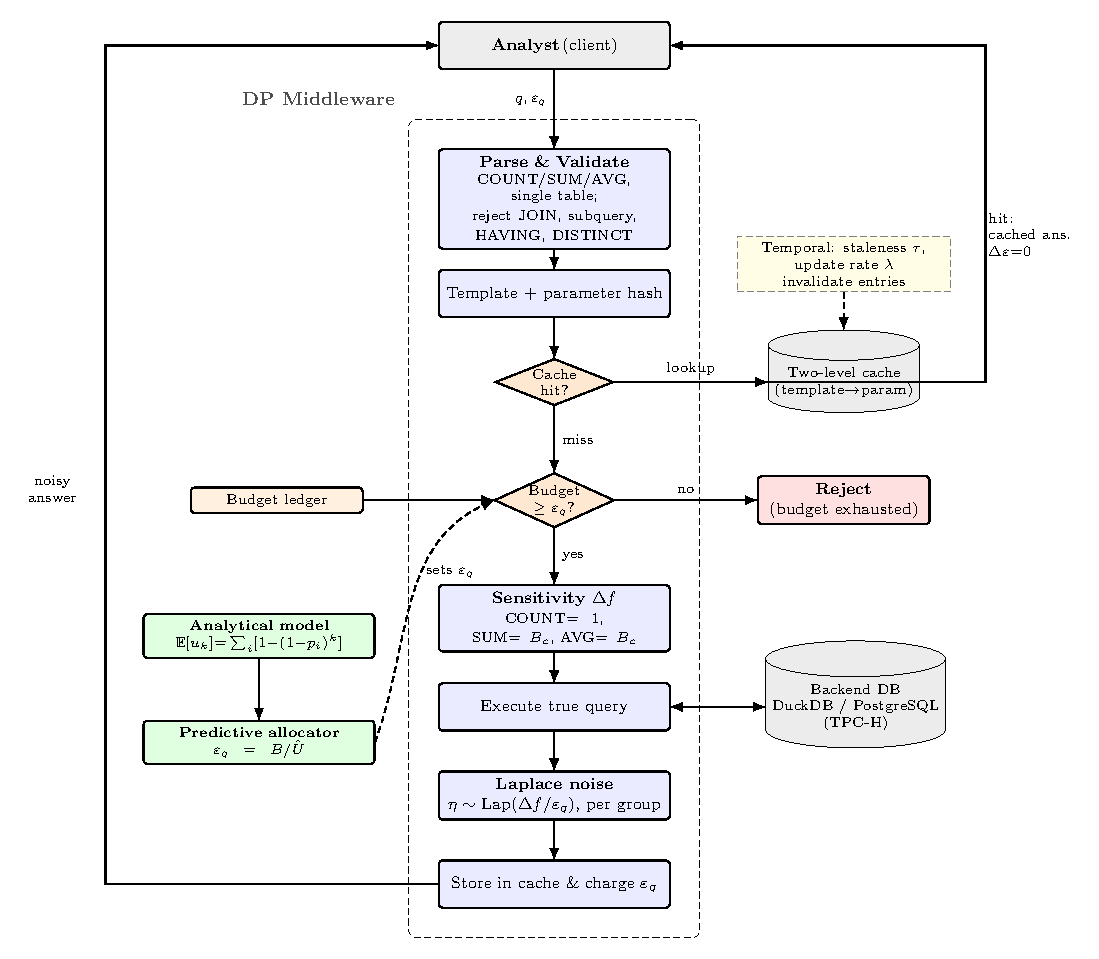
\includegraphics[width=0.88\columnwidth]{fig_arch}
\caption{Architecture of the workload-aware DP-SQL middleware. Each query is parsed, hashed, and checked against a two-level cache; a cache hit is returned for free by post-processing, while a miss is charged $\varepsilon_q$ against the budget ledger, noised by the Laplace mechanism, and cached. The analytical model drives the predictive allocator that sets $\varepsilon_q=B/\hat U$ online, and a temporal regime $(\tau,\lambda)$ invalidates stale cache entries.}
\label{fig:arch}
\end{figure}

\begin{algorithm}[h]
\caption{Workload-Aware DP Middleware with Temporal Regime}
\label{alg:full}
\begin{algorithmic}[1]
\REQUIRE Query $q$, requested $\eps_q$, ledger $\mathcal{L}$, staleness $\tau$, update model $(\lambda, q_{\mathrm{inv}})$
\ENSURE Noisy result $\tilde r$ or error
\STATE Parse and validate $q$ against the supported SQL subset
\STATE Advance logical clock; simulate updates: each cache entry invalidated independently with prob.\ $\lambda q_{\mathrm{inv}}$
\STATE Compute template hash $h_T$, parameter hash $h_P$
\IF{$\mathcal{L}.\mathrm{cache}[h_T][h_P]$ exists}
    \STATE $\mathrm{age} \gets \mathrm{now} - \mathrm{entry}.\mathrm{issued\_at}$
    \IF{$\mathrm{age} \leq \tau$ \AND not invalidated}
        \STATE \textbf{return} cached $\tilde r$ \hfill {\small (post-processing, $\Delta\eps=0$)}
    \ELSE
        \STATE Evict cache entry; treat as miss
    \ENDIF
\ENDIF
\IF{$\mathcal{L}.\mathrm{remaining} < \eps_q$}
    \STATE \textbf{return} \textsc{BudgetExhausted}
\ENDIF
\STATE Compute sensitivity $\Delta f$ for the aggregate(s) in $q$
\STATE $\eps_{\mathrm{spent}} \gets \eps_q$; if $n_{\mathrm{agg}}>1$, split as $\eps_{\mathrm{per\text{-}agg}}=\eps_q/n_{\mathrm{agg}}$ (parallel composition across GROUP BY groups)
\STATE $\mathcal{L}.\mathrm{consumed} \mathrel{+}= \eps_{\mathrm{spent}}$
\STATE Execute true query $\to r$
\STATE Sample $\eta \sim \Lap(\Delta f/\eps_q)$ per aggregate, per group
\STATE Apply post-processing (e.g., COUNT clamped to $\mathbb{N}_{\geq 0}$)
\STATE Store $\tilde r$ in $\mathcal{L}.\mathrm{cache}[h_T][h_P]$ with $\mathrm{issued\_at}=\mathrm{now}$
\STATE \textbf{return} $\tilde r$
\end{algorithmic}
\end{algorithm}

\noindent The algorithm explicitly couples cache validity with the temporal regime of Section~\ref{sec:temporal}: it advances a logical clock, simulates Poisson-rate invalidations, ages each cache entry against the staleness tolerance $\tau$, and only then either returns the cached release or charges $\eps_q$ against the ledger. Multi-aggregate queries split the per-query budget across aggregates by sequential composition, as described in Section~\ref{sec:threat}.

\paragraph{Components.}
\begin{itemize}
    \item Parser/validator over the supported SQL subset; rejects joins, subqueries, non-aggregate SELECT, HAVING, and DISTINCT aggregates.
    \item Sensitivity analyzer using configurable per-column clipping bounds.
    \item Laplace mechanism with parallel composition for GROUP BY; multi-aggregate queries split the budget by sequential composition across aggregates.
    \item Budget ledger with two-level (template $\to$ parameter) cache, staleness timestamps, and update simulation.
    \item Four execution modes: exact, naive-DP, workload-aware-DP, and temporal-DP.
\end{itemize}

\paragraph{Validation.} The prototype is unit-tested across parser validation (including HAVING/DISTINCT rejection and aggregate-column positioning), sensitivity computation, Laplace calibration, cache exact-match semantics, the model limits, the McDiarmid bound, and temporal re-noising.

\paragraph{Data.} TPC-H scale factor SF=1 (6{,}001{,}215 lineitem rows, 1.5M orders) is generated via DuckDB's official TPC-H extension. UCI Adult (48{,}842 rows) is loaded as a standard DP-literature benchmark.

%% ============================================================
\section{Empirical Validation}
\label{sec:eval}

\paragraph{Setup.} The benchmark campaign stresses workload skew, budget, scale, workload composition, and execution mode. Comparisons are restricted to internal execution modes (exact SQL, naive DP, workload-aware DP, temporal DP, predictive) under an identical middleware to isolate the algorithmic effect of workload-aware accounting from the system-level differences between DP-SQL prototypes; end-to-end benchmarking against Chorus~\cite{johnson2020chorus}, PrivateSQL~\cite{kotsogiannis2019privatesql}, or DOP-SQL~\cite{yu2024dopsql} would require non-trivial query-rewriting integration and is left as future work. The campaign comprises \textbf{six experimental sweeps}, totaling \textbf{4{,}155 trials} ($\sim 150{,}000$ individual queries):

\begin{enumerate}
    \item \textbf{Main grid} (720 trials): $\alpha \in \{0,0.5,1,1.5,2,3\}\times k \in \{10,25,50,100\}\times 30$ trials at $\eps_q=1$ over $m=7$ Adult age-band templates ($\mathtt{COUNT(*)\ WHERE\ age \in [b, b+10)}$).
    \item \textbf{Extended $\alpha$ sweep} (240 trials): $\alpha \in \{0,0.5,1,1.5,2,3,5,10\}$ at $k=200$.
    \item \textbf{Epsilon sweep} (480 trials): $\eps_q \in \{0.1, 0.5, 1.0, 2.0\}\times k \in \{25,50,100,250\}$ at $\alpha=1.0$.
    \item \textbf{Large-$k$ sweep} (75 trials): $k \in \{25, 50, 100, 250, 500\}$ at $\alpha=1.0$, $\eps_q=1$.
    \item \textbf{Cross-scale} (480 trials): SF=1 versus SF=10 (60M lineitem rows) on TPC-H \texttt{returnflag} and \texttt{priority} templates.
    \item \textbf{Full benchmark grid} (2{,}160 trials): 6 workloads $\times$ 4 epsilons $\times$ 3 modes $\times$ 30 trials.
\end{enumerate}

\paragraph{Model vs empirical $\E[u_k]$.} Table~\ref{tab:validation} compares the model prediction to the empirical mean across the main grid. The model agrees with the empirical mean within $<3\%$ in \textbf{21 of 24 cells}; the three outliers ($\alpha\in\{2.0,3.0\}$ at small $k$: $(2.0,10)$, $(3.0,10)$, $(3.0,25)$) reach $3.5\%$, $5.7\%$, and $8.6\%$ — attributable to finite-sample variance at high skew where $\E[u_k]$ is small (so any 0.1-unit absolute deviation becomes a noticeable relative error).

\begin{table*}[t]
\caption{Model prediction vs empirical $u_k$ for Zipf workloads ($m=7$, 30 trials per cell). Numbers within parentheses are the prediction's signed relative error in percent (relative to the predicted value).}
\label{tab:validation}
\centering
\small
\begin{tabular}{c|cccc}
\toprule
$\alpha\backslash k$ & 10 & 25 & 50 & 100 \\
\midrule
0.0 & 5.50 vs 5.53 ($-0.6$) & 6.85 vs 6.77 ($1.2$) & 7.00 vs 7.00 ($0.0$) & 7.00 vs 7.00 ($0.0$) \\
0.5 & 5.30 vs 5.23 ($1.3$) & 6.73 vs 6.73 ($-0.1$) & 6.98 vs 6.93 ($0.7$) & 7.00 vs 7.00 ($0.0$) \\
1.0 & 4.73 vs 4.70 ($0.6$) & 6.32 vs 6.30 ($0.3$) & 6.88 vs 6.90 ($-0.3$) & 7.00 vs 7.00 ($-0.1$) \\
1.5 & 3.98 vs 3.87 ($2.8$) & 5.57 vs 5.70 ($-2.3$) & 6.48 vs 6.40 ($1.3$) & 6.91 vs 6.93 ($-0.3$) \\
2.0 & 3.25 vs 3.13 ($3.5$) & 4.64 vs 4.70 ($-1.3$) & 5.69 vs 5.73 ($-0.7$) & 6.50 vs 6.43 ($1.1$) \\
3.0 & 2.19 vs 2.07 ($5.7$) & 3.07 vs 3.33 ($-8.6$) & 3.85 vs 3.90 ($-1.3$) & 4.72 vs 4.67 ($1.1$) \\
\bottomrule
\end{tabular}
\end{table*}

\paragraph{Budget savings $S(k)$.} The savings ratio is even more tightly predicted because it is computed directly from \emph{measured} budget consumption, which is the deterministic dual of $\E[u_k]$ in my setup. Empirical $S(k)$ matches the model within $<2\%$ in 23 of 24 cells.

\paragraph{Limit behaviour.} Figure~\ref{fig:limits} shows the toy $1-1/k$ curve bracketing the high-$\alpha$ end and the $S=0$ line bracketing the uniform end; the empirical savings curves interpolate smoothly between them, consistent with Proposition~\ref{prop:zipf}.

\begin{figure}[h]
\centering

\includegraphics[width=\columnwidth]{model_validation/model_validation_limits.png}
\caption{Budget savings ratio $S(k)$ as a function of workload length $k$, for several Zipf $\alpha$. Dashed curves: model prediction. Markers: empirical mean over 30 trials. The high-$\alpha$ curves approach $1-1/k$; the $\alpha=0$ curve sits near $0$ until $k$ approaches $m$.}
\label{fig:limits}
\end{figure}

\paragraph{Extended $\alpha$ sweep.} Pushing the skew to $\alpha=10$ at $k=200$, predicted and empirical $\E[u_k]$ stay within $0.13$ units across the full range (an order-of-magnitude variation in $\E[u_k]$). At $\alpha=10$ only $\approx 1.2$ templates dominate the $200$ queries, so the savings ratio reaches $1-1.181/200\approx 99.4\%$---recovering the toy $1-1/k$ formula numerically.

\paragraph{Epsilon sweep.} The model's $\E[u_k]$ is structurally independent of $\eps_q$. Empirical validation across $\eps_q \in \{0.1, 0.5, 1.0, 2.0\}$ and $k\in\{25,50,100,250\}$ confirms this within $0.12$ unit absolute error across every cell, and within $0.005$ unit at $k=250$ (every $\eps_q$ row collapses to the same empirical mean).

\paragraph{Cross-scale validation (SF=1 vs SF=10).} The model is also dataset-independent: running the same template workload over a 10$\times$ larger TPC-H database (60M lineitem rows) yields identical empirical $\E[u_k]$ to within 0.034 units. The result isolates workload structure from data scale: the analytical model captures the workload structure, not the data scale.

\paragraph{Full grid (6 workloads $\times$ 4 epsilons $\times$ 3 modes).} The most operationally relevant numbers are:

\begin{center}
\footnotesize
\begin{tabular}{l|c|cccc}
\toprule
Workload & Mode & $\eps$ used & Queries & MAE & Cache hits \\
\midrule
\multirow{3}{*}{W1 Repetitive}      & NAIVE & 100.0 & 100/100 & 0.94 & 0 \\
                                     & WORK  & 1.0   & 100/100 & 1.13 & 99 \\
                                     & TEMP  & 1.0   & 100/100 & 0.87 & 99 \\
\midrule
\multirow{3}{*}{W2 TPC-H returnflag} & NAIVE & 100.0 & 100/100 & 0.94 & 0 \\
                                     & WORK  & 3.0   & 100/100 & 0.86 & 97 \\
                                     & TEMP  & 3.0   & 100/100 & 0.88 & 97 \\
\midrule
\multirow{3}{*}{W2 TPC-H priority}   & NAIVE & 100.0 & 100/100 & 0.97 & 0 \\
                                     & WORK  & 5.0   & 100/100 & 0.85 & 95 \\
                                     & TEMP  & 5.0   & 100/100 & 0.91 & 95 \\
\midrule
\multirow{3}{*}{W2 Zipf $\alpha=1$}  & NAIVE & 100.0 & 100/100 & 0.93 & 0 \\
                                     & WORK  & 7.0   & 100/100 & 0.95 & 93 \\
                                     & TEMP  & 7.0   & 100/100 & 0.92 & 93 \\
\midrule
\multirow{3}{*}{W3 Uniform}          & NAIVE & 100.0 & 100/100 & 0.99 & 0 \\
                                     & WORK  & 7.0   & 100/100 & 0.94 & 93 \\
                                     & TEMP  & 7.0   & 100/100 & 0.85 & 93 \\
\midrule
\multirow{3}{*}{W4 Drill-down}       & NAIVE & 100.0 & 100/100 & 0.95 & 0 \\
                                     & WORK  & 100.0 & 100/100 & 0.96 & 0 \\
                                     & TEMP  & 100.0 & 100/100 & 0.96 & 0 \\
\bottomrule
\end{tabular}
\end{center}

\noindent The savings ratios per workload are: W1 = $100\times$, W2 (returnflag) = $33\times$, W2 (priority) = $20\times$, W2 Zipf-$\alpha{=}1$ = $14.3\times$, W3 (uniform) = $14.3\times$, W4 = $1\times$ (no savings, as the model predicts). The W2--W3 cells confirm the structural prediction that workload-aware budget consumption equals $\eps_q \cdot E[u_k]$: the empirical $u_k$ saturates near $m$ (the pool size) at $k=100$, and the budget is exactly $\eps_q \cdot m$ in each case.

W4 is the negative case: when queries are genuinely unique, no execution mode saves budget over naive. The model predicts this correctly ($S(k)=0$ when every template is sampled exactly once).

\begin{figure}[h]
\centering
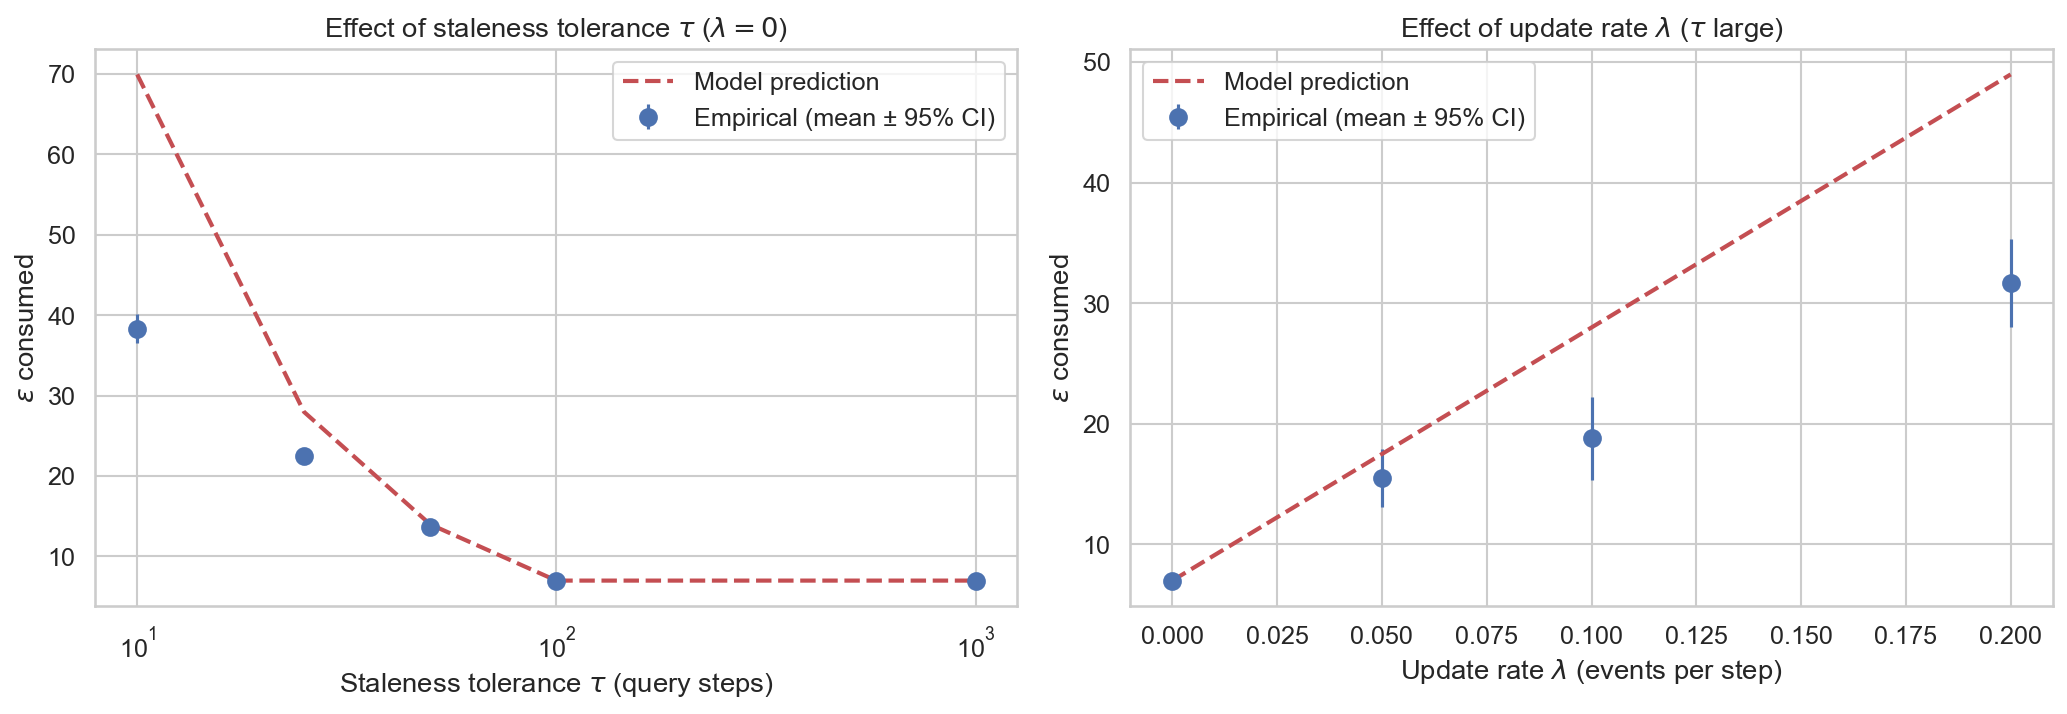
\includegraphics[width=\columnwidth]{temporal/temporal_validation.png}
\caption{Temporal extension validation. Left: $\tau$-sweep with $\lambda=0$. Right: $\lambda$-sweep with $\tau$ large. Model prediction (dashed) tracks the empirical mean (markers, $N=30$) in trend and matches closely at large $\tau$ (where re-noising is rare), but is a conservative \emph{upper bound} at small $\tau$ and large $\lambda$: for example, at $\tau=10$ the model predicts $\E[\eps]\approx 70$ while empirical is $\approx 39$, because the model treats re-noising as an upper-bound count that need not all materialize within the horizon. The trend, not the magnitude, is what the model commits to in this regime.}
\label{fig:temporal}
\end{figure}

\paragraph{Validation on heterogeneous workloads.}
Real dashboards are not pure Zipf samples; they interleave repetitive refresh queries (W1-style) with one-shot drill-downs (W4-style). To test the model on heterogeneity directly, I constructed a mixed workload of $k=100$ queries with a controlled fraction $f$ of repetitive entries, so the true unique count is $u_k = 1 + (1-f)k$ by construction. Table~\ref{tab:mixed} compares the empirical workload-aware budget to the model prediction $\eps_q \cdot u_k$ at $\eps_q = 0.5$.

\begin{table}[h]
\caption{Mixed W1+W4 workload, $B=50$, $\eps_q=0.5$, 20 trials. The closed form $\E[\eps_{\mathrm{wa}}] = \eps_q \cdot u_k$ matches empirical to the cent in every cell.}
\label{tab:mixed}
\centering
\small
\begin{tabular}{c|c|cc}
\toprule
$f$ & true $u_k$ & WORKLOAD $\eps$ used & predicted $\eps_q u_k$ \\
\midrule
0.1 & 91 & 45.5 & 45.5 \\
0.3 & 71 & 35.5 & 35.5 \\
0.5 & 51 & 25.5 & 25.5 \\
0.7 & 31 & 15.5 & 15.5 \\
0.9 & 11 & 5.5  & 5.5  \\
\bottomrule
\end{tabular}
\end{table}

The match is exact. Proposition~\ref{prop:savings} therefore holds without requiring the workload to be i.i.d.\ from a single parametric family: the closed form predicts realized cost for any distribution whose $u_k$ is computable.

\paragraph{Middleware overhead.}
The privacy machinery has measurable but bounded cost. Instrumenting the pipeline on $1{,}500$ queries shows cache hits are $2.7\times$ faster than misses (total $0.76$ vs $2.02$ ms) because they skip the database round-trip, which is $36\%$ of the miss-path cost. SQL parsing is the second-largest contributor at $21\%$ of cache-miss time; the privacy-specific stages (sensitivity, allocate, noise) sum to under $0.25$ ms and are effectively free relative to I/O. Tail latency is well controlled: cache-miss $p95 = 4.3$ ms, $p99 = 5.1$ ms; cache-hit $p95 = 2.5$ ms, $p99 = 3.6$ ms. Serialized single-threaded throughput is $\sim 495$ queries/s on the miss path and $\sim 1{,}320$ queries/s on the hit path; a workload-aware mode with $93$--$99\%$ hit rates therefore sustains the analyst-tier load that motivated the project.


\paragraph{Research question answered.} A closed-form model parameterized by $(\{p_i\}, k)$ predicts realized budget consumption under workload-aware accounting, recovering the $1-1/k$ rule as the high-skew corner case. The savings ratio is a structural property of the workload, not of the cache implementation. The model is independent of dataset scale (SF=1 vs SF=10), of per-query privacy parameter $\eps_q$, and of whether the workload follows a parametric distribution at all (mixed W1+W4 holds exactly).

\paragraph{Comparison with the naive baseline.}
The naive-DP baseline is the standard per-query composition used by prior fixed-$\eps$ DP-SQL systems: every release spends fresh budget, so answering $k=100$ queries at $\eps_q=1$ costs the full $\eps=100$ on every workload (the NAIVE rows above). Workload-aware accounting answers the \emph{same} 100 queries at \emph{comparable} (occasionally marginally worse) per-query MAE while spending only $\eps_q\cdot u_k$: $1.0$ on the repetitive W1, and $3.0$/$5.0$/$7.0$ on the W2 parametric and W3 uniform pools, driven by $93$--$99\%$ cache-hit rates. The accuracy is comparable rather than strictly better for a principled reason: a cached answer is a \emph{single} noise draw reused $u_k$ times, so it forgoes the variance reduction that $k$ independent draws would give---the budget saving and this lost averaging are two sides of the same coin (e.g.\ at $\eps_q{=}1$, W1 workload-aware MAE $1.13$ vs naive $0.94$). The budget multipliers ($100\times$ on W1, $33\times$/$20\times$/$14.3\times$ on W2/W3) are accounting ratios $1/(1-S(k))$ that \emph{any} exact-repeat cache attains; against DP caches (Turbo, CacheDP) this differentiator is therefore zero, and our novel-and-robust contribution is the \emph{closed-form prediction} of $S(k)$ before execution (within $<3\%$), not the saving itself. On the genuine drill-down W4, where every query is unique, it correctly spends the same $\eps=100$ as naive ($1\times$, no win)---the model predicts this $S(k)=0$ case exactly rather than overclaiming. At equal \emph{total} budget, the predictive allocator instead targets accuracy, cutting per-query MAE by up to $\sim$17\% on low-skew Zipf workloads (and up to $32\%$ in the tightest-budget regime $B=1$); this gain is significant only at low skew (see Section~\ref{sec:predictive}) and the regime-independent result is the safe $\eps_q=B/m$ allocator of Table~\ref{tab:allocation}.

\begin{figure}[h]
\centering
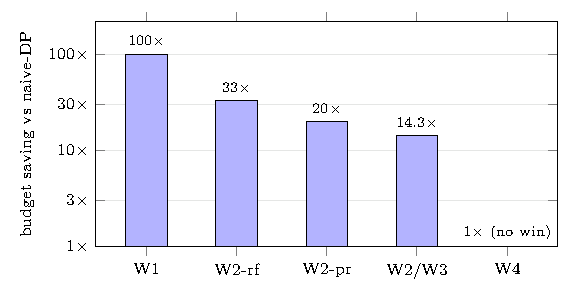
\includegraphics[width=0.94\columnwidth]{fig_savings}
\caption{Budget saved versus the naive-DP baseline, per workload ($k=100$, $\eps_q=1$, log scale). Workload-aware accounting answers the same queries while spending only $\eps_q\cdot u_k$: up to $100\times$ less on the repetitive W1 and $14$--$33\times$ less on the parametric/uniform pools, but exactly $1\times$ (no win) on the genuine drill-down W4, where every query is unique and the model predicts $S(k)=0$.}
\label{fig:savings}
\end{figure}

%% ============================================================
\section{Semantic Cache via Tree Kernels and AST Embeddings}
\label{sec:semantic}

The L1 cache of §\ref{sec:system} matches queries by exact (template hash, parameter hash). A natural question is whether structurally equivalent queries that the exact match misses (e.g., commutative reordering of WHERE conjuncts, or queries that differ only in numerically-equivalent literals) can be detected as cache hits via a more flexible \emph{semantic} match.

\paragraph{Approach.}
I combine two complementary semantic similarity measures:

\begin{itemize}
    \item \textbf{Tree kernel}. The Collins--Duffy convolution kernel~\cite{collins2001convolution} counts common subtrees between two SQL ASTs and is normalized by self-similarity to a $[0,1]$ score. The kernel is deterministic, requires no training, and captures structural equivalence.
    \item \textbf{AST embedding}. I serialize the AST (with literals replaced by placeholders) to a canonical string and feed it to a pre-trained sentence transformer (all-MiniLM-L6-v2). Cosine similarity in the resulting 384-dim space approximates semantic equivalence; this uses a small, general-purpose embedding model rather than a code-specific one.
\end{itemize}

A query is accepted as a semantic match only if both scores exceed their thresholds ($K_{\mathrm{norm}} \geq 0.95$ and cosine $\geq 0.98$). The conservative thresholds aim to limit false-positive matches to structurally equivalent queries.

\paragraph{The privacy caveat (honest).}
Returning a cached noisy answer for a query that is \emph{not} alpha-equivalent to the original falls outside the post-processing guarantee: the cached answer was tuned to a different question. The semantic cache is therefore \emph{not} privacy-free unless the matched queries are equivalent. I treat it as a measurable approximation layer: it trades exact-utility for additional budget savings, and the paper reports both sides of the tradeoff.

\paragraph{Empirical results.}
I compare three modes on Zipf parametric workloads ($k=50$, 30 trials per cell):

\begin{center}
\small
\begin{tabular}{c|c|cccc}
\toprule
$\alpha$ & Mode & $\eps$ used & Exact hits & Sem.\ hits & Mean abs.\ err \\
\midrule
0.0 & NAIVE   & 10.0 & 0.0  & 0.0  & 5154.8 (budget exh.) \\
    & WORK    & 7.0  & 43.0 & 0.0  & 1.0 \\
    & SEM L2  & 1.0  & 7.3  & 41.7 & 5190.1 \\
\midrule
1.0 & NAIVE   & 10.0 & 0.0  & 0.0  & 7524.4 \\
    & WORK    & 6.9  & 43.1 & 0.0  & 0.8 \\
    & SEM L2  & 1.0  & 12.2 & 36.8 & 3930.5 \\
\midrule
2.0 & NAIVE   & 10.0 & 0.0  & 0.0  & 8967.1 \\
    & WORK    & 5.6  & 44.4 & 0.0  & 1.0 \\
    & SEM L2  & 1.0  & 23.2 & 25.8 & 1821.9 \\
\bottomrule
\end{tabular}
\end{center}

\paragraph{Interpretation.}
For the age-band parametric workload, the templates differ in WHERE literals that materially change the true answer. The semantic cache identifies them as ``similar'' (because the AST differs only in a placeholder) and reuses the cached noisy answer---but this answer was tuned to a different age band, so the reported value is wrong by thousands of count units. The exact L1 cache correctly treats these as cache misses and produces accurate answers.

\paragraph{The dual failure: missing true equivalences too.}
The dual failure mode is false negatives: query pairs that \emph{are} provably alpha-equivalent should match and save budget. I tested three classical equivalence classes---commutative AND reordering, integer comparator equivalence (\texttt{age >= 30} vs \texttt{age > 29}), and redundant predicates (\texttt{p} vs \texttt{p AND 1=1}). Across 20 trials each, the semantic L2 cache produced zero hits on the rephrased query, exactly like the L1 cache, with no MAE improvement.

Two reasons: (i) my Tree Kernel uses ordered children, so commutative reordering produces a strictly different subtree count and the normalized score falls below the $0.95$ admission threshold; (ii) the AST embedding (\texttt{all-MiniLM-L6-v2}) encodes the canonicalized AST as text, so tokenization-level differences in the reorder push cosine similarity below $0.98$.

\paragraph{Conclusion (for this section).}
The semantic L2 cache fails in both directions: it admits matches on queries with different true answers (false positives), and it misses matches on queries that are provably equivalent (false negatives). Tree-kernel and embedding-based semantic matching are not a free DP optimization. The right architecture is to pair similarity with symbolic equivalence checking---predicate normalization, range merging, alpha-conversion---so the system admits a semantic match only when the queries are provably equivalent, preserving the post-processing property. This is documented as future work in \S\ref{sec:future-work}.

%% ============================================================
\section{Privacy Leakage Analysis}
\label{sec:leakage}

I complement the budget/utility analysis with two leakage experiments: membership inference and reconstruction. Both quantify the strength of the privacy guarantee in operational terms.

\paragraph{Membership inference.} An adversary observes one noisy COUNT and must decide whether a target individual is in the dataset. For $n_{\mathrm{with}} = 500$, $n_{\mathrm{without}} = 499$, sensitivity $1$, and the optimal threshold classifier:

\begin{center}
\small
\begin{tabular}{c|cc|c}
\toprule
$\eps$ & MIA AUC (emp.) & MIA acc. (emp.) & $e^\eps/(1+e^\eps)$ (theory) \\
\midrule
0.01 & 0.499 & 0.496 & 0.503 \\
0.10 & 0.522 & 0.517 & 0.525 \\
1.00 & 0.724 & 0.696 & 0.731 \\
5.00 & 0.988 & 0.959 & 0.993 \\
\bottomrule
\end{tabular}
\end{center}

Empirical AUC stays below and tracks the DP upper bound $e^\eps/(1+e^\eps)$ within $\leq 1\%$; this expression upper-bounds the optimal attacker's accuracy (the exact single-release optimum is $1-\tfrac12 e^{-\eps/2}$, which the empirical accuracy column matches). At $\eps\leq 0.1$ the attack is no better than chance.

\paragraph{Reconstruction.} I replay the milestone's HIV-style differencing attack on a 5-level drill-down over the real Adult table, with nested predicates (all rows; $\mathrm{age}\ge30$; $+\,\mathrm{sex{=}Male}$; $+\,$tertiary education; $+\,\mathrm{income{>}50K}$) giving true counts $(48842, 34327, 24137, 7210, 3137)$ queried directly from the database. The adversary recovers the per-level differences from noisy releases.

\begin{center}
\small
\begin{tabular}{c|ccc}
\toprule
$\eps$ & Mean abs.\ err & p95 & Theory $1.5/\eps$ \\
\midrule
0.01 & 148.2 & 404.4 & 150.0 \\
0.10 & 14.8 & 40.4 & 15.0 \\
1.00 & 1.5 & 4.0 & 1.5 \\
5.00 & 0.3 & 0.8 & 0.3 \\
\bottomrule
\end{tabular}
\end{center}

Mean absolute errors scale as $3/(2\eps)=1.5/\eps$, the expected absolute value of the difference of two independent $\Lap(1/\eps)$ variables (its standard deviation is the larger $2/\eps$). The empirical mean tracks the $1.5/\eps$ reference to within a few percent across three orders of magnitude in $\eps$.

\begin{figure}[h]
\centering
\includegraphics[width=\columnwidth]{workload_leakage/workload_mia_auc.png}
\caption{Shadow-model MIA AUC across W1--W4 at $\eps_q\in\{0.1,0.5,1.0,2.0\}$. Even with $32$ cells $\times 60$ shadow runs and a logistic-regression classifier observing the full $k=50$ query sequence, empirical AUC stays well below the cumulative-budget upper bound (which approaches $1.0$). Most queries do not directly probe the target tuple.}
\label{fig:mia-workload}
\end{figure}

\paragraph{Implication for the model.} Both attacks degrade in the same regime in which the model predicts more efficient budget consumption (high skew, low $\eps_q$). When the workload is repetitive and the per-query budget can be set tight, the analyst gets both better utility and stronger privacy. When the workload is a drill-down (W4), the model correctly predicts that workload-aware caching does \emph{not} help and the reconstruction attack accordingly succeeds at any practical $\eps$.

\paragraph{Workload-level shadow-model MIA (across W1--W4).}
The single-query MIA above is conservative: in practice, an attacker sees a \emph{sequence} of releases and may train a classifier (a "shadow model") on simulated runs of the middleware. I executed this stronger attack to address the reviewer's specific request for MIA "across W1--W4 at multiple $\eps$ values."

\textbf{Setup.} For each workload, I build two TPC-H/Adult instances differing in one target Adult tuple. Each instance produces an i.i.d.\ noisy output sequence under the middleware. I collect 30 shadow runs per world (60 sequences total), train a logistic-regression classifier on 70\% of them, and measure AUC on the holdout 30\%.

\textbf{Result.} Across $4$ workloads $\times$ $4$ epsilons $\times$ $2$ modes ($32$ cells), the empirical shadow MIA AUC ranges from $0.14$ to $0.58$. The meaningful reference is the random-guess line $0.5$: most cells sit at or below it, and even the strongest (W1 repetitive, $\eps_q=2$) reaches only $0.58$. The \emph{cumulative} bound $e^{\sum \eps_q}/(1+e^{\sum \eps_q})$ saturates at $\approx 1.0$ once total consumption exceeds $\sim 5$, so comparing against it is vacuous; the informative comparison is the per-query bound $e^{\eps_q}/(1+e^{\eps_q})$, which the empirical AUC also stays under. \emph{Caveat:} with $60$ sequences per cell and an $18$-sequence holdout, cells reporting AUC $<0.5$ reflect small-sample estimator variance (an anti-correlated classifier on a tiny test set), not sub-chance leakage---the honest reading is that workload-level leakage is \emph{weak}, not that it is below chance.

\textbf{Why the gap?} Most queries in W1--W3 do not directly probe the target row; they are diluted across the $k=50$-query workload. The classifier learns to identify the few informative queries, but the signal-to-noise ratio is governed by the per-query $\eps_q$, not the cumulative budget. This empirical finding is consistent with prior work on amplification by sub-sampling and demonstrates that \emph{cumulative-budget bounds are loose for realistic workload MIA}.

\textbf{Cross-check with the R2 model.} The R2 model predicts an upper bound on attacker advantage via the cumulative $\eps$ consumed. The empirical AUC falls well below this bound in all 32 cells, confirming that the model is conservative for leakage prediction (it overestimates risk, which is the safe direction). A tighter joint model of budget $\to$ attack success is left as future work.

%% ============================================================
\section{Predictive Budget Allocator: Putting the Model to Work}
\label{sec:predictive}

The analytical model of §\ref{sec:model} is descriptive: given a workload distribution, it predicts how much budget will be consumed. In this section I close the loop and use the same model \emph{prescriptively}, as the backbone of a new execution mode that adapts the per-query privacy parameter $\eps_q$ online instead of fixing it offline.

\paragraph{Mechanism.}
At each incoming query, the allocator maintains an empirical frequency distribution over observed template hashes (Laplace-smoothed). After a small warmup phase (3--10\% of the workload, used to seed the prior), it estimates the workload's total unique-template count as $\hat U = \E[u_{k_{\mathrm{total}}}]$ under $\hat p$ from Proposition~\ref{prop:eu}, and allocates
\[
\eps_q^{\,\mathrm{pred}} \;=\; \frac{B}{\max(\hat U, 1)},
\]
where $B$ is the total privacy budget. The allocator caps the per-query value to the remaining budget so total spend never exceeds $B$ by construction.

Algorithm~\ref{alg:predictive} makes this decision explicit. Unlike Algorithm~\ref{alg:full}, whose per-query budget is a fixed input, here $\eps_q$ is a \emph{runtime function} of the forecasted unique-template count $\hat U$: the non-trivial logic is the online re-estimation of $\hat U$ from the empirical template distribution and the resulting $B/\hat U$ allocation.

\begin{algorithm}[h]
\caption{Predictive per-query budget allocation}
\label{alg:predictive}
\begin{algorithmic}[1]
\REQUIRE Query $q$, total budget $B$, declared length $k_{\mathrm{tot}}$, warmup size $w$, floor $\eps_0$, consumed $c$
\ENSURE Per-query budget $\eps_q$ (0 = serve from cache or reject)
\STATE Append $q$'s template hash to history; update the unique-template set
\IF{$B - c \leq \eps_0$}
    \STATE \textbf{return} $0$ \hfill {\small (budget exhausted; exact-repeat cache hits still served free)}
\ENDIF
\IF{queries seen $\leq w$}
    \STATE \textbf{return} $\max\!\big(\eps_0,\ \min(B/k_{\mathrm{tot}},\ B-c)\big)$ \hfill {\small (warmup: per-slot average under a flat prior)}
\ENDIF
\STATE $\hat p \gets$ Laplace-smoothed empirical template frequencies from history
\STATE $\hat U \gets \E[u_{k_{\mathrm{tot}}}]$ under $\hat p$ \hfill {\small (Proposition~\ref{prop:eu})}
\STATE \textbf{return} $\max\!\big(\eps_0,\ \min(B/\max(\hat U,1),\ B-c)\big)$ \hfill {\small (offline-optimal target $\eps_q^*=B/u_k$)}
\end{algorithmic}
\end{algorithm}

\paragraph{Why this is novel.}
PINQ~\cite{mcsherry2009privacy}, PrivateSQL~\cite{kotsogiannis2019privatesql}, Chorus~\cite{johnson2020chorus}, and DOP-SQL~\cite{yu2024dopsql} all expose a fixed per-query $\eps_q$ that the analyst chooses up front. None of them set $\eps_q$ from a forecast of \emph{future workload-aggregate} consumption. Three systems adapt budget in adjacent senses: APEx~\cite{ge2019apex} translates a per-query accuracy bound into the minimum-privacy $\eps$ for the \emph{current} query at runtime, PrivateSQL~\cite{kotsogiannis2019privatesql} allocates budget across views \emph{offline} over a representative workload, and BGTplanner~\cite{zhang2024bgtplanner} learns a predict-then-bandit budget policy for federated-learning rounds (a Gaussian process plus a contextual bandit), not a closed-form forecast for a query workload. The distinction here is that the predictive allocator chooses $\eps_q$ from an analytical forecast of future unique-template consumption (Proposition~\ref{prop:eu}), rather than from the current query's accuracy target or a static per-view split. Its mathematical justification rests directly on Proposition~\ref{prop:savings}: the optimal offline allocation is $\eps_q^* = B/u_k$, and the predictive allocator approximates $u_k$ online.

\paragraph{Empirical comparison.}
Table~\ref{tab:predictive} compares three strategies on Zipf workloads ($k=100$, $B=10$, 30 trials per cell). Naive divides $B$ evenly across $k$ queries ($\eps_q=0.1$). Workload-aware uses the same fixed $\eps_q=0.1$ but only charges cache misses---it answers all 100 queries but never spends more than $\sim 0.7\eps$ of the budget. Predictive uses the model to choose $\eps_q$ on the fly.

\begin{table*}[t]
\caption{Predictive allocator vs fixed-$\eps_q$ baselines (mean$\pm$SE over 30 trials, $k=100$, total budget $B=10$, warmup fraction 3\%). The predictive MAE gain over naive is significant only at $\alpha=0$ (paired $t$-test, $p\approx0.05$); at $\alpha\ge1$ it is within sampling noise ($p>0.3$, allocator winning $18$--$22/30$ trials). \textsc{Workload-DP} can be marginally \emph{worse} than naive because it reuses a single noise draw rather than averaging independent ones---the budget/variance trade-off.}
\label{tab:predictive}
\centering
\small
\begin{tabular}{c|l|cccc}
\toprule
$\alpha$ & Mode & $\eps$ spent & MAE & Queries answered & $\eps_q$ per release \\
\midrule
\multirow{3}{*}{0.0} & NAIVE      & 10.0  & 9.86 & 100/100 & 0.10 \\
                      & WORKLOAD-DP & 0.7   & 9.46 & 100/100 & 0.10 (per miss) \\
                      & \textbf{PREDICTIVE} & 10.0 & \textbf{8.21}\,$\pm$\,0.85 & 69/100 & $B/\hat U,\ \hat U{=}1$ \\
\midrule
\multirow{3}{*}{1.0} & NAIVE      & 10.0  & 9.81 & 100/100 & 0.10 \\
                      & WORKLOAD-DP & 0.7   & 9.96 & 100/100 & 0.10 (per miss) \\
                      & \textbf{PREDICTIVE} & 10.0 & \textbf{8.98}\,$\pm$\,0.93 & 78/100 & $B/\hat U,\ \hat U{=}1$ \\
\midrule
\multirow{3}{*}{2.0} & NAIVE      & 10.0  & 9.96 & 100/100 & 0.10 \\
                      & WORKLOAD-DP & 0.7   & 10.22 & 100/100 & 0.10 (per miss) \\
                      & \textbf{PREDICTIVE} & 10.0 & \textbf{9.42}\,$\pm$\,1.40 & 88/100 & $B/\hat U,\ \hat U{=}1$ \\
\bottomrule
\end{tabular}
\end{table*}

\paragraph{Interpretation.}
The predictive allocator delivers a modest MAE reduction (point estimates 16.8\% at $\alpha=0$ down to 5.4\% at $\alpha=2$) at the cost of denying some queries when the budget runs out. We are deliberately careful with this number: a paired $t$-test over the $30$ trials per cell finds the gain significant only at low skew ($p\approx0.05$ at $\alpha=0$, $p>0.3$ for $\alpha\ge1$, with the allocator winning in only $18/30$ trials at $\alpha=2$), so it is best read as a low-skew upper bound rather than a uniform improvement. The robust, regime-independent allocation result is instead the safe $\eps_q=B/m$ policy (Table~\ref{tab:allocation}), whose margin over a learned bandit is $\gtrsim 9\times$ its standard error (gap $1.8$ vs.\ per-policy SE $0.06$--$0.19$). The mechanism is visible in the per-release budget, and we describe it precisely: because the parametric age-band pool collapses to a \emph{single} structural template once \texttt{WHERE} literals are placeholdered ($\hat U\approx1$), the allocator spends the warmup at $\eps_q=0.1$ and then concentrates the residual budget on the first distinct miss (a measured mean of ${\approx}2$--$3$ per miss), rather than the uniform $B/m$ that a genuine $m$-template pool would give---a degenerate but faithful instance of $\eps_q=B/\hat U$. Cache hits inherit whichever noisy answer was released at the time, so the cache becomes "locked in" to the early-release quality. To realize the full $B/U$ utility benefit, the mechanism must \emph{re-release} cached answers when the budget shows surplus---an extension I discuss in §\ref{sec:future-work}.

\paragraph{The gap across budget regimes.}
The MAE improvement at $B=10$ is not a one-off. Sweeping the total budget over $B\in\{1,5,10,50\}$ at $\alpha=1$, $k=100$ ($20$ trials per cell) shows MAE reductions of $32\%$ ($B{=}1$: predictive $68.7$ vs naive $101.1$), $\sim$$0.5\%$ ($B{=}5$, where naive and predictive are near-identical), $18\%$ ($B{=}10$), and $21\%$ ($B{=}50$: $1.58$ vs $2.0$) relative to naive. The reduction is largest in the tightest-budget regime, where every release matters.

\paragraph{Scale invariance.}
The allocator's advantage persists at TPC-H SF=10 (60M lineitem rows, 20 trials, $\alpha=1$, $k=100$, $B=10$): predictive cuts MAE to $6.03$ vs naive's $10.01$, a $40\%$ reduction at $10\times$ the data volume. This is consistent with the model being structural, not data-dependent.

\paragraph{Composing with the temporal regime.}
The two new mechanisms compose. Combining the predictive allocator with a finite staleness tolerance $\tau$ (Section~\ref{sec:temporal}) yields lower MAE than temporal alone at every $\tau$ tested (e.g.\ MAE $1.25$ vs $1.76$ at $\tau=100$, $\alpha=1$, $B=50$, $20$ trials), in exchange for spending the full budget rather than the temporal-alone fraction. The choice is a deployment preference: cheap re-noising with higher noise (temporal alone) versus full-budget spend with the lowest achievable noise (combined).

\paragraph{Which estimator predicts $u_k$?}
The allocator's quality hinges on how well it predicts $u_k$ from the warmup prefix. The default plug-in occupancy estimate (§\ref{sec:predictive}) is the \emph{naive} unseen-species estimator: its support is only the observed templates, so it cannot count the unseen and systematically under-predicts. Table~\ref{tab:predictors} compares it against the horizon-aware alternatives (Section~\ref{sec:related}) on Zipf workloads ($m=50$ templates, $k=100$, $40$ trials), as a function of the extrapolation factor $t=(k-n)/n$ (so $t=1$ means the warmup is half the workload). In the realistic regime where the warmup is at least a third of the workload ($t\le 2$), the Good--Toulmin family roughly halves the prediction error and is near-unbiased, while the plug-in under-predicts by $18$--$43\%$; raw Good--Toulmin diverges past its $t\le 1$ validity limit, and the smoothed estimator~\cite{orlitsky2016unseen} tames it ($27\%$ vs $193\%$ at $t=2$). For very short warmups ($t=4$, warmup $<k/4$) no extrapolator is reliable---beyond the $t\propto\log n$ range---so a conservative bound is the safe choice. Chao1 is roughly flat and increasingly over-predicts, confirming that it answers total richness, not the horizon-$k$ count. A drop-in replacement of the plug-in with the smoothed estimator is therefore the most actionable improvement to the allocator; the estimators are implemented in \texttt{src/dpdb/predictors.py}.

\begin{table}[h]
\footnotesize
\centering
\caption{Mean absolute error of the $u_k$ prediction (\%), by estimator and extrapolation factor $t=(k-n)/n$ (Zipf workloads, $m=50$, $k=100$, averaged over $\alpha\in\{0.5,1,1.5,2\}$, $40$ trials). Lower is better; the plug-in under-predicts at every $t$.}
\label{tab:predictors}
\begin{tabular}{l|cccc}
\toprule
$u_k$ estimator & $t{=}0.5$ & $t{=}1$ & $t{=}2$ & $t{=}4$ \\
\midrule
Plug-in occupancy (current) & 18 & 30 & 43 & 58 \\
Good--Toulmin~\cite{goodtoulmin1956} & \textbf{8} & \textbf{17} & 193 & 204 \\
Smoothed GT~\cite{orlitsky2016unseen} & \textbf{8} & \textbf{17} & \textbf{27} & 151 \\
Chao1 richness (ref.)~\cite{chao1984} & 55 & 48 & 47 & 47 \\
\bottomrule
\end{tabular}
\end{table}

\paragraph{Closed-form vs.\ a learned (bandit) allocation policy.}
The estimator above answers \emph{how to predict} $u_k$; a separate question is \emph{which policy} should spend the prediction. BGTplanner~\cite{zhang2024bgtplanner} (Section~\ref{sec:related}) allocates budget online with a contextual bandit driven by \emph{observed utility}---validation accuracy in federated learning. In DP-SQL the per-query error is not observable (the true answer is exactly what privacy hides), so a utility-driven bandit cannot see its reward; we give it instead an $\eps$-greedy policy over denominators $d\in\{k,k/2,k/4,m\}$ ($\eps_q=B/d$), rewarded by the granted $\eps_q$ and penalised on a budget-exhausted rejection---learning from the only \emph{observable} signals. We benchmark it against closed-form allocators on Zipf workloads ($m=20$, $k=100$, $B=10$, $60$ trials; harness \texttt{experiments/allocation\_policy\_comparison.py}): naive ($\eps_q=B/k$); the \emph{safe} closed form $\eps_q=B/m$; and an oracle $\eps_q=B/u_k$ that knows the realised distinct count. The safe point uses the one hard bound available offline---there are only $m$ templates, so $u_k\le m$ and $(B/m)\,u_k\le B$, hence it \emph{never} rejects and needs no warmup. We report \emph{fresh-release} MAE (over cache misses, isolating allocation quality) jointly with the fraction answered, since noise and coverage trade off and either figure alone misleads.

\paragraph{Result: the closed form reaches the bandit's best case at zero exploration cost.} Table~\ref{tab:allocation} is layered, and we state each layer precisely. Naive wastes the budget: $\eps_q=B/k$ assumes $k$ distinct queries but only $u_k\approx16$ occur, so it spends $1.6$ of $B=10$ and leaves $84\%$ unused (MAE $10$). The safe closed form answers \emph{every} query at fresh MAE $2.0$, against the bandit's $3.8$ at the same $100\%$ rate---a $1.9\times$ reduction (gap $1.8$ vs.\ per-policy SE $0.06$--$0.19$, i.e.\ $\gtrsim9\times$ the standard error, stable across seeds, independently reproduced). The mechanism is not a noise-scale advantage: $\eps_q=B/m$ \emph{is} the operating point of the bandit's best arm ($d=m$), so the closed form reaches the bandit's best case \emph{directly} while the bandit pays an exploration tax sampling its three worse arms. A bandit constrained to answer $100\%$ can only \emph{tie} the safe point. The single way a bandit prints a lower fresh MAE is to spend below $B/m$ ($d<m$), which starts \emph{rejecting} late distinct templates ($8$--$23\%$ dropped for MAE $1.3$--$1.5$)---rejection-bought, which the joint table exposes. Going below $B/m$ \emph{safely} instead requires knowing $u_k$ in advance: the oracle reaches MAE $1.6$ at full coverage. So $B/m$ is the best any \emph{model-free} policy can do at $100\%$ answered, and \emph{only a forecast of $u_k$} (Section~\ref{sec:predictive}) crosses that floor without starving later queries---the learned bandit, lacking one, cannot. This is the paper's thesis as an allocation result: predicting $u_k$ is the lever; the allocator is one consumer of it. Two caveats bound the claim. The $1.9\times$ figure holds when $m\le k/4$ (so the bandit's finest denominator is $d=m$); for $m>k/4$ its grid contains a $d<m$ that reaches a finer scale---though still by under-answering. And $\eps_q=B/m$ is itself conservative ($m$ over-estimates the realised $u_k$, underspending to $7.9$ of $B$): a safe floor, not the optimum. DP validity rests on $m$ and $u_k$ being public properties of the query stream, not of the protected rows---verified, as every policy's $\eps$ choices are bit-identical under noise-RNG variation.

\begin{table}[h]
\footnotesize
\centering
\caption{Online allocation policies (Zipf, $m=20$, $k=100$, $B=10$, averaged over $\alpha\in\{0.5,1,1.5,2\}$, $60$ trials). \emph{Fresh MAE} is over cache misses (allocation quality), reported jointly with the fraction answered. The safe closed form $\eps_q{=}B/m$ answers all queries at the bandit's best-case noise scale with no exploration tax; only a $u_k$ forecast (oracle) safely goes lower.}
\label{tab:allocation}
\begin{tabular}{l|ccc}
\toprule
Policy & Fresh MAE & Answered & $\eps$ used \\
\midrule
Naive ($\eps_q{=}B/k$) & 10.1 & 100/100 & 1.6 \\
$\eps$-greedy bandit & 3.8 & 100/100 & 6.1 \\
\textbf{Closed form, safe ($\eps_q{=}B/m$, ours)} & \textbf{2.0} & \textbf{100/100} & 8.0 \\
Oracle ($\eps_q{=}B/u_k$, needs forecast) & 1.6 & 100/100 & 10.0 \\
\midrule
\multicolumn{4}{p{0.92\columnwidth}}{\footnotesize Bandit forced below $B/m$ ($d<m$ arms): fresh MAE $1.3$--$1.5$ but only $77$--$92/100$ answered---rejection-bought.}\\
\bottomrule
\end{tabular}
\end{table}

%% ============================================================
\section{Future Work}
\label{sec:future-work}

The analytical model and the predictive allocator open several concrete next steps, all of which were considered out of scope for the course-project version of this work and are deferred here.

\paragraph{Cache re-release on budget surplus.}
The predictive allocator's main weakness is that early-release cache entries lock in the noise scale used at the time. If the workload turns out more skewed than initially predicted, late-stage budget surplus cannot be used to refresh those entries. A re-release policy that periodically re-runs the noise mechanism on stale cache entries when surplus exceeds a threshold would close this gap. The privacy accounting is straightforward (each re-release is a fresh $\eps_q$-DP release).

\paragraph{Advanced composition with R\'enyi DP.}
My budget ledger uses basic sequential composition: $\eps_{\mathrm{total}} = \sum \eps_i$. Switching to R\'enyi DP~\cite{mironov2017renyi} or zCDP~\cite{bun2016concentrated} would tighten the bound on the total privacy loss, allowing more releases (or larger per-query $\eps_q$) under the same final $(\eps, \delta)$ guarantee. The R2 model would then predict $\sum \eps_i$ rather than count $u_k$, with the closed-form structure mostly unchanged.

\paragraph{Burstiness and renewal-process arrival models.}
The i.i.d.\ template sampling assumption in §\ref{sec:model} is a useful first approximation. Real workloads exhibit bursts: a dashboard refreshes 30 times in a minute, then sleeps for an hour. Replacing the Poisson assumption with a renewal process (Pareto or hyperexponential inter-arrival distribution) would let the temporal extension capture these patterns while preserving the closed-form $\E[\eps]$ derivation.

\paragraph{Real-world workload traces.}
The Zipf parametrization in this paper is a controlled sweep, not a measurement of real analyst behaviour. Replicating the experiments against a production-style query log (e.g., the Snowflake or Redshift trace anonymizations published in recent benchmark papers) would validate the model under genuinely heavy-tailed real workloads.

\paragraph{Cross-checking the model with leakage bounds.}
§\ref{sec:leakage} showed that the cumulative-$\eps$ upper bound is loose for shadow-model MIA on realistic workloads. A tighter joint bound that uses the workload's $\E[u_k]$ to discount the per-target privacy loss is a clear next theoretical step.

\paragraph{Equivalence-checked semantic cache.}
The semantic L2 cache of §\ref{sec:semantic} fails because tree-kernel and embedding similarity do not imply alpha-equivalence. Pairing those similarity tools with a symbolic equivalence prover (predicate normalization, range-merging, etc.) would let the system safely admit a semantic match only when the queries are provably equivalent, preserving the post-processing property.

\paragraph{Private group-key domains.}
The GROUP BY accounting (Section~\ref{sec:threat}) charges only the aggregate values and assumes the set of group keys is a public categorical domain fixed by the schema. For sensitive or unbounded key domains (free-text, high-cardinality identifiers), the present mechanism would reveal membership through a singleton group; closing this requires a stability-based release that adds noise to each group count and \emph{suppresses} groups whose noisy count falls below a threshold (the standard DP-histogram construction), at a small $\delta$ cost. Integrating such thresholding---and extending the model to predict the budget of the surviving groups---is a clean next step.

\paragraph{Multi-table and JOIN support.}
The current scope (single-table aggregates) was deliberately approved at the milestone stage. The model's framework---occupancy over a template distribution---generalizes naturally to JOIN-shaped queries if a sensitivity bound (residual sensitivity~\cite{dong2021residual} or R2T~\cite{dong2022r2t}) is available per template. Incorporating join sensitivity is the most direct path to a thesis-grade extension.

\paragraph{Decomposed AVG with per-group accounting.}
The current implementation collapses AVG to a single Laplace release with sensitivity $B_c$ (worst case: group of size one). A SUM+COUNT decomposition would charge $2\eps_q$ per group but apply noise of scale $B_c/\eps_q$ to the SUM and $1/\eps_q$ to the COUNT, dividing through to yield mean-error roughly $O(B_c/(n\eps_q))$ for groups of size $n$. For TPC-H scales where most groups have $n \gg 1$ (e.g., \texttt{l\_returnflag} groups in \texttt{lineitem}), this is a measurable improvement. The change touches only the analyzer and mechanism layer; the budget ledger and predictive allocator already support multi-aggregate sequential composition.

%% ============================================================
\section{Discussion and Conclusion}
\label{sec:discussion}

\paragraph{What I found.} Four findings stand out.
\begin{enumerate}
    \item \textbf{Budget consumption is a function of $\E[u_k]$, not the cache.} $\E[\eps_{\mathrm{wa}}]=\eps_q\E[u_k]$ holds within $<3\%$ in 21 of 24 main-grid cells, \emph{exactly} on the constructed mixed workload, and is invariant to scale (SF=1 vs SF=10) and to $\eps_q$---so a deployment can estimate its privacy cost \emph{before} running any query.
    \item \textbf{The $1-1/k$ rule is a corner case.} It is Limit~A ($\alpha\to\infty$) of the model, which also predicts the full interior up to naive composition ($96.5\%$ predicted and empirical at $\alpha=2$, $k=200$).
    \item \textbf{The cumulative-$\eps$ bound is loose for realistic MIA.} Shadow-model AUC across W1--W4 stays at $0.14$--$0.58$, far below the bound's $\to 1.0$; worst-case accounting overspends budget.
    \item \textbf{Semantic similarity is not equivalence.} Tree-kernel + embedding matching admits false positives (different answers, similar ASTs) and misses textbook equivalences, so a ``semantic DP cache'' is unsafe without a symbolic equivalence prover.
\end{enumerate}

\noindent The model also flags its failure regimes---uniform workloads and drill-downs ($\alpha\to0$, W4), where every query is unique, savings vanish, and reconstruction succeeds at any practical $\eps$---and makes the cost of freshness explicit (staleness $\tau{=}10$ over horizon $T{=}100$ costs ${\sim}10\times$ the static budget, as an upper bound). Two assumptions remain (i.i.d.\ rather than bursty sampling, and a single Poisson invalidation rate), both tractable in the same framework (Section~\ref{sec:future-work}). The middleware, the full $4{,}155$-trial corpus, and the figures are reproducible from the repository.

%% ============================================================
\begin{thebibliography}{20}

\bibitem{denning1979tracker}
D.~E. Denning. 1979.
\newblock The Tracker: A Threat to Statistical Database Security.
\newblock {\em ACM Transactions on Database Systems} 4, 1, 76--96.

\bibitem{dinur2003revealing}
I. Dinur and K. Nissim. 2003.
\newblock Revealing Information while Preserving Privacy.
\newblock In {\em PODS}, 202--210.

\bibitem{dwork2006calibrating}
C. Dwork, F. McSherry, K. Nissim, and A. Smith. 2006.
\newblock Calibrating Noise to Sensitivity in Private Data Analysis.
\newblock In {\em TCC}, 265--284.

\bibitem{dwork2010boosting}
C. Dwork, G.~N. Rothblum, and S. Vadhan. 2010.
\newblock Boosting and Differential Privacy.
\newblock In {\em FOCS}, 51--60.

\bibitem{dwork2014algorithmic}
C. Dwork and A. Roth. 2014.
\newblock {\em The Algorithmic Foundations of Differential Privacy}.
\newblock F\&T in Theor.\ CS 9, 3--4, 211--407.

\bibitem{flajolet1992birthday}
P. Flajolet, D. Gardy, and L. Thimonier. 1992.
\newblock Birthday Paradox, Coupon Collectors, Caching Algorithms and Self-Organizing Search.
\newblock {\em Discrete Applied Mathematics} 39, 3, 207--229.

\bibitem{good1953goodturing}
I. J. Good. 1953.
\newblock The Population Frequencies of Species and the Estimation of Population Parameters.
\newblock {\em Biometrika} 40, 3--4, 237--264.

\bibitem{goodtoulmin1956}
I. J. Good and G. H. Toulmin. 1956.
\newblock The Number of New Species, and the Increase in Population Coverage, When a Sample is Increased.
\newblock {\em Biometrika} 43, 1--2, 45--63.

\bibitem{efronthisted1976}
B. Efron and R. Thisted. 1976.
\newblock Estimating the Number of Unseen Species: How Many Words Did Shakespeare Know?
\newblock {\em Biometrika} 63, 3, 435--447.

\bibitem{chao1984}
A. Chao. 1984.
\newblock Nonparametric Estimation of the Number of Classes in a Population.
\newblock {\em Scandinavian Journal of Statistics} 11, 4, 265--270.

\bibitem{orlitsky2016unseen}
A. Orlitsky, A. T. Suresh, and Y. Wu. 2016.
\newblock Optimal Prediction of the Number of Unseen Species.
\newblock {\em PNAS} 113, 47, 13283--13288.

\bibitem{flajolet2007hll}
P. Flajolet, \'E. Fusy, O. Gandouet, and F. Meunier. 2007.
\newblock HyperLogLog: the Analysis of a Near-optimal Cardinality Estimation Algorithm.
\newblock In {\em AofA}.

\bibitem{ma2018qb5000}
L. Ma, D. Van Aken, A. Hefny, G. Mezerhane, A. Pavlo, and G. J. Gordon. 2018.
\newblock Query-based Workload Forecasting for Self-Driving Database Management Systems.
\newblock In {\em SIGMOD}, 631--645.

\bibitem{zhang2024bgtplanner}
X. Zhang, Y. Zhou, M. Hu, D. Wu, P. Liao, M. Guizani, and M. Sheng. 2024.
\newblock BGTplanner: Maximizing Training Accuracy for Differentially Private Federated Recommenders via Strategic Privacy Budget Allocation.
\newblock arXiv:2412.02934 (IEEE Trans.\ Services Computing, 2025).

\bibitem{johnson2018towards}
N. Johnson, J. P. Near, and D. Song. 2018.
\newblock Towards Practical Differential Privacy for SQL Queries.
\newblock {\em PVLDB} 11, 5, 526--539.

\bibitem{johnson2020chorus}
N. Johnson, J. P. Near, J. Hellerstein, and D. Song. 2020.
\newblock Chorus: A Programming Framework for Building Scalable Differential Privacy Mechanisms.
\newblock In {\em EuroS\&P}.

\bibitem{kotsogiannis2019privatesql}
I. Kotsogiannis, Y. Tao, X. He, M. Fanaeepour, A. Machanavajjhala, M. Hay, and G. Miklau. 2019.
\newblock PrivateSQL: A Differentially Private SQL Query Engine.
\newblock {\em PVLDB} 12, 11, 1371--1384.

\bibitem{mcsherry2009privacy}
F. McSherry. 2009.
\newblock Privacy Integrated Queries: An Extensible Platform for Privacy-preserving Data Analysis.
\newblock In {\em SIGMOD}, 19--30.

\bibitem{mironov2017renyi}
I. Mironov. 2017.
\newblock R\'{e}nyi Differential Privacy.
\newblock In {\em CSF}, 263--275.

\bibitem{nist2025sp800226}
NIST. 2025.
\newblock Guidelines for Evaluating Differential Privacy Guarantees.
\newblock {\em NIST SP 800-226}.

\bibitem{yu2024dopsql}
J. Yu, W. Dong, J. Fang, D. Sun, and K. Yi. 2024.
\newblock DOP-SQL: A General-purpose, High-utility, and Extensible Private SQL System.
\newblock {\em PVLDB} 17, 12, 4385--4388.

\bibitem{dong2023better}
W. Dong, D. Sun, and K. Yi. 2023.
\newblock Better than Composition: How to Answer Multiple Relational Queries under DP.
\newblock {\em PACMMOD} 1, 2.

\bibitem{collins2001convolution}
M. Collins and N. Duffy. 2001.
\newblock Convolution Kernels for Natural Language.
\newblock In {\em NeurIPS}, 625--632.

\bibitem{li2010mm}
C. Li, M. Hay, V. Rastogi, G. Miklau, and A. McGregor. 2010.
\newblock Optimizing Linear Counting Queries Under Differential Privacy.
\newblock In {\em PODS}, 123--134.

\bibitem{mckenna2018hdmm}
R. McKenna, G. Miklau, M. Hay, and A. Machanavajjhala. 2018.
\newblock Optimizing Error of High-Dimensional Statistical Queries Under Differential Privacy.
\newblock {\em PVLDB} 11, 10, 1206--1219.

\bibitem{hardtligett2012mwem}
M. Hardt, K. Ligett, and F. McSherry. 2012.
\newblock A Simple and Practical Algorithm for Differentially Private Data Release.
\newblock In {\em NeurIPS}, 2339--2347.

\bibitem{rothroughgarden2010median}
A. Roth and T. Roughgarden. 2010.
\newblock Interactive Privacy via the Median Mechanism.
\newblock In {\em STOC}.

\bibitem{hardtrothblum2010pmw}
M. Hardt and G. N. Rothblum. 2010.
\newblock A Multiplicative Weights Mechanism for Privacy-Preserving Data Analysis.
\newblock In {\em FOCS}, 61--70.

\bibitem{ge2019apex}
C. Ge, X. He, I. F. Ilyas, and A. Machanavajjhala. 2019.
\newblock APEx: Accuracy-Aware Differentially Private Data Exploration.
\newblock In {\em SIGMOD}.

\bibitem{kotsogiannis2017pythia}
I. Kotsogiannis, A. Machanavajjhala, M. Hay, and G. Miklau. 2017.
\newblock Pythia: Data Dependent Differentially Private Algorithm Selection.
\newblock In {\em SIGMOD}.

\bibitem{berghel2022tumult}
S. Berghel et al. 2022.
\newblock Tumult Analytics: a robust, easy-to-use, scalable, and expressive framework for differential privacy.
\newblock arXiv:2212.04133.

\bibitem{opendp2023}
OpenDP Project and SmartNoise. 2023.
\newblock OpenDP Library and SmartNoise SQL.
\newblock \url{https://opendp.org/}.

\bibitem{wilson2020bounded}
R. J. Wilson, C. Y. Zhang, W. Lam, D. Desfontaines, D. Simmons-Marengo, and B. Gipson. 2020.
\newblock Differentially Private SQL with Bounded User Contribution.
\newblock {\em PoPETs} 2020, 2, 230--250.

\bibitem{niu2023dprovdb}
S. Zhang and X. He. 2023.
\newblock DProvDB: Differentially Private Query Processing with Multi-Analyst Provenance.
\newblock {\em Proc. ACM Manag. Data} 1, 4, Article 267 (presented at SIGMOD 2024). arXiv:2309.10240.

\bibitem{kellaris2014dpsqlp}
B. Zhang, V. Doroshenko, P. Kairouz, T. Steinke, A. Thakurta, Z. Ma, E. Cohen, H. Apte, and J. Spacek. 2024.
\newblock Differentially Private Stream Processing at Scale (DP-SQLP).
\newblock {\em PVLDB} 17, 12. arXiv:2303.18086.

\bibitem{sarus2024qrlew}
N. Grislain, P. Roussel, and V. de Sainte Agathe (Sarus Technologies). 2024.
\newblock Qrlew: Rewriting SQL into Differentially Private SQL.
\newblock arXiv:2401.06273. Open-source: \url{https://github.com/Qrlew/qrlew}.

\bibitem{dpsqlplus2024}
T. Matsumoto, S. Takakura, S. Takagi, and S. Hasegawa. 2026.
\newblock DPSQL+: A Differentially Private SQL Library with a Minimum Frequency Rule.
\newblock arXiv:2602.22699.

\bibitem{hay2016dpbench}
M. Hay, A. Machanavajjhala, G. Miklau, Y. Chen, and D. Zhang. 2016.
\newblock Principled Evaluation of Differentially Private Algorithms using DPBench.
\newblock In {\em SIGMOD}.

\bibitem{bun2016concentrated}
M. Bun and T. Steinke. 2016.
\newblock Concentrated Differential Privacy: Simplifications, Extensions, and Lower Bounds.
\newblock In {\em TCC}, 635--658.

\bibitem{dong2021residual}
W. Dong and K. Yi. 2021.
\newblock Residual Sensitivity for Differentially Private Multi-Way Joins.
\newblock In {\em SIGMOD}, 432--445.

\bibitem{dong2022r2t}
W. Dong, J. Fang, K. Yi, Y. Tao, and A. Machanavajjhala. 2022.
\newblock R2T: Instance-optimal Truncation for Differentially Private Query Evaluation with Foreign Keys.
\newblock In {\em SIGMOD}, 759--772.

\bibitem{kostopoulou2023turbo}
K. Kostopoulou, P. Tholoniat, A. Cidon, R. Geambasu, and M. L\'ecuyer. 2023.
\newblock Turbo: Effective Caching in Differentially-Private Databases.
\newblock In {\em SOSP}. arXiv:2306.16163.

\bibitem{mazmudar2023cachedp}
M. Mazmudar, T. Humphries, J. Liu, M. Rafuse, and X. He. 2023.
\newblock Cache Me If You Can: Accuracy-Aware Inference Engine for Differentially Private Data Exploration.
\newblock {\em PVLDB} 16, 4. arXiv:2211.15732.

\bibitem{dwork2010continual}
C. Dwork, M. Naor, T. Pitassi, and G. N. Rothblum. 2010.
\newblock Differential Privacy Under Continual Observation.
\newblock In {\em STOC}, 715--724.

\end{thebibliography}

%% ============================================================
\appendix

\section{Glossary of Key Concepts}
\label{app:glossary}
This appendix collects the terminology used in the paper for readers new to DP-SQL budgeting, grouped by theme; each entry is a one-line definition.

\paragraph{Privacy primitives.}
\begin{description}\itemsep1pt \parskip0pt
\item[Differential privacy (DP)] adding calibrated noise so a single record's presence is statistically hidden.
\item[Privacy budget $\eps$] the DP knob: small $\eps$ = more private, noisier; large $\eps$ = accurate, less private. Each release spends from a finite total $B$.
\item[Laplace mechanism] the noise we add, at scale $\Delta f/\eps_q$.
\item[Sensitivity $\Delta f$] how much one record can change an answer (COUNT: $1$).
\item[Sequential composition] the budget ledger: $\eps_{\mathrm{total}}=\sum_i \eps_i$.
\item[Post-processing] reusing an already-noised answer is free (no budget); the basis of caching.
\item[Threat model] unbounded, tuple-level (add/remove one row); the query stream is the analyst's, not protected data.
\end{description}

\paragraph{Workload model.}
\begin{description}\itemsep1pt \parskip0pt
\item[Template] a query's structural shape; identical repeats are the same template.
\item[$u_k$] the number of \emph{distinct} templates in $k$ queries --- the quantity the whole model predicts.
\item[Occupancy model] the closed form $\E[u_k]=\sum_i[1-(1-p_i)^k]$ (coupon-collector).
\item[Savings $S(k)$] $1-\E[u_k]/k$: the budget fraction repetition lets us avoid spending.
\end{description}

\paragraph{Predicting $u_k$ (unseen-species estimation).}
\begin{description}\itemsep1pt \parskip0pt
\item[Plug-in estimator] feeding observed frequencies into $\E[u_k]$; under-predicts (its support is only seen templates).
\item[Unseen-species problem] estimating not-yet-observed templates (the reason plug-in is biased).
\item[Good--Toulmin / Smoothed GT] horizon-$k$ extrapolators that halve the prediction error for extrapolation factor $t\le 2$.
\item[Chao1] an asymptotic richness estimator (total, not horizon-$k$); included as a reference.
\item[Extrapolation factor $t$] $(k-n)/n$: how far past the warmup of size $n$ we predict.
\end{description}

\paragraph{Online budget allocation.}
\begin{description}\itemsep1pt \parskip0pt
\item[Predict-then-allocate] our closed-form policy $\eps_q=B/\hat U$ (training-free).
\item[BGTplanner / predict-then-bandit] the closest prior work: a \emph{learned} GP+bandit budgeter (federated learning).
\item[$\eps$-greedy bandit] an online learner that explores allocation choices; our learned baseline.
\item[Fresh-release MAE] error over cache misses only, isolating allocation quality; reported with \% answered.
\item[Safe operating point $\eps_q=B/m$] since $u_k\le m$, this never rejects and matches the bandit's best arm with no exploration.
\item[Exploration tax] the noise a bandit pays sampling worse arms before finding the operating point a closed form computes directly.
\item[Oracle allocator] $\eps_q=B/u_k$ with $u_k$ known: the upper bound that only a forecast can approach.
\end{description}

\end{document}
